\documentclass{llncs}

\usepackage{graphicx}
\usepackage{biblatex}
\usepackage{caption}
\usepackage[english]{babel}
\usepackage{caption}
\usepackage{subcaption}
\usepackage{csquotes}
\usepackage{multirow}
\usepackage{nth}

\makeatletter
\newcommand*{\rom}[1]{\expandafter\@slowromancap\romannumeral #1@}
\makeatother

\setlength{\textfloatsep}{7pt}
\setlength{\floatsep}{5pt}
\setlength{\intextsep}{7pt}
\newcommand{\squeezeup}{\vspace{-2.5mm}}

\addbibresource{literature.bib}

\begin{document}

\title{Fault Classification of Rotating Machinery using Limited Set of Features and k-Nearest Neighbors}

\author{
	Miroslav Hájek\thanks{Master study programme in field: Informatics,
	Supervisor: Dr. Marcel Baláž, Institute of Computer Engineering and Applied Informatics, Faculty of Informatics and Information Technologies STU in Bratislava}
}

\institute{Faculty of Informatics and Information Technologies STU in Bratislava\\
\email{xhajekm@stuba.sk}}

\maketitle

\begin{abstract}
The ability to detect and diagnose faulty parts of the machine is important for the industry at scale. Continuous monitoring of vibrations  with accelerometers used as a diagnostic tool demands significant requrements for bandwidth and storage of samples. Standards already establish reliable attributes for the fault presence. The same cannot be said for purposes of root cause analysis. The goal is to examine the effect of reducing the number of features for fault prediction accuracy in the k-nearest neighbor model. We extract ten features in the time domain and eleven in frequency domain in the MaFaulDa dataset. We compare the accuracy of the whole feature set with three member subsets chosen by brute force, PCA, and feature selection methods: correlation, f-statistic, mutual information, and their rank product. We also qualitatively analyze features from the vibrations of water pumps. The rank product reaches accuracy 83.90\% and 79.08\%, for the time and frequency domain, respectively, which is by 1.82\% and 5.13\% less than the best three-member subset found by brute force.

\keywords{feature selection \and machine fault diagnosis \and vibrations \and MaFaulDa \and k-NN}
\end{abstract}


\section{Introduction}
Rotary motion machinery is utilized throughout the industry as motors, pumps, and gearboxes. All equipment has a bounded productive lifespan because of wear and tear or improper operating conditions. Sooner or later, moving elements start to exhibit faults that can lead to failure if left untreated. 

Early real-time fault detection can be achieved by monitoring machine vibration levels and signal frequency content~\cite{ziaran_technicka_2013}. Sensors for vibrations are piezoelectric or MEMS wideband accelerometers. Data acquisition procedures and best evaluation practices are standardized in ISO~20816~\cite{noauthor_iso_2016} and ISO~13373~\cite{noauthor_iso_2002}. 

Such a monitoring solution with the Internet of Things devices allows us to introduce predictive (PdM) or condition-based maintenance (CbM). This strategy prolongs the life of the equipment and reduces the cost of replacement parts and preventive maintenance~\cite {ziaran_technicka_2013}. 

A large number of machines in the plant and frequent sampling intervals pose a challenge with the sheer amount of samples gathered. Data reduction should happen close to the source to save on storage requirements, and bandwidth and promote retainment of important observations only. An additional difficulty is to tailor the fault classification model to individual machinery because each piece has natural imperfections and differences in its construction. 

Technical diagnosis identifies faulty machinery parts that can be bearings, shafts, coupling, belts, or gear. The commonly found defects are imbalance, misalignment, looseness, eccentricity, deformation, crack, and rub~\cite{mohanty_machinery_2015, scheffer_practical_2004}. Most symptoms in vibrations appear synchronous to the rotational speed of the component under investigation as fundamental frequency of rotation or its harmonics~\cite{davies_handbook_2012}. Multiple faults can arise simultaneously or induce one another. For example, a severely damaged bearing introduces shaft imbalance.

\section{Related work}
Approaches taken in literature to reduce vibration samples and classify faults result in a similar framework of machine learning pipeline. The general sequence of steps consists of signal acquisition, feature extraction, dimensionality reduction, and pattern recognition or fault detection~\cite{wang_bearing_2015, brito_fault_2021}. 

Data retrieval from acceleration sensors is supplemented by a factory database of machinery mechanical parameters and operating conditions~\cite{jung_vibration_2017}. The signal processing methods extract low-level numerical features in the time domain, frequency domain, and time-frequency domain~\cite{nandi_condition_2019}. Time-frequency features depend on the transform method of which Morlet wavelet transform, discrete wavelet transform, or wavelet packet transform are the ones used besides short-time Fourier transform~\cite{maurya_condition-based_2021}. Then, statistical functions such as root mean square, centroid, kurtosis, energy, and entropy are applied to further compress the waveform. 

Feature extraction of time and frequency domain attributes is utilized in online monitoring of band saw blade wear status from acoustic emission signal using SVM model ~\cite{zhuo_research_2022} and in novelty detection of health status of centrifugal pump using autoencoder~\cite{mostafavi_novel_2021}. Wavelength length, average amplitude change, and zero crossing taken out of overview of time domain features for surface electromyography (sEMG)~\cite{moctar_time-domain_2023} are generic enough to be tried for machine diagnostic. Harmonic features originally designed for sound description~\cite{peeters_large_2004} could be reused similarly. Many features found in the literature are already implemented in the Time Series Feature Extraction Library (TSFEL) which is a package for Python language~\cite{tsfel}. 

Knowledge of rolling bearings geometry and rotational speed provides a way to calculate bearing defect frequencies for outer race (BPFO), inner race (BPFI), ball (BSF), and cage (FTF)~\cite{mohanty_machinery_2015, ziaran_technicka_2013}. There are situations when bearing fault is not evidenced by defect frequency. Therefore, kurtosis is recommended as it is associated with impacts~\cite{brito_fault_2021}.

Normalization assigns the same weights to unbounded variables~\cite{zheng_feature_2018}. In three-dimensional motion, either axis aligned only with the principal direction of vibrations is retained, or the Euclidian norm is computed for each feature. The idea of feature vector magnitude comes from animal activity recognition based on collar tags independent of sensor orientation~\cite{kamminga_robust_2018}. 

Extracted features lower the number of dimensions from the original signal. Further dimensionality reduction is carried out with various methods: PCA, t-SNE, ISOMAP, ICA, and AE~\cite{brito_fault_2021}. Keeping a smaller number of attributes can result in better classification performance. However, the major disadvantage is the lack of meaning in acquired features. 

Filtering feature selection methods decrease the feature set size so that the chosen predictors are related the strongest to a categorical predicted variable.
The relationship is quantified with correlation, fisher score, or mutual information and among others~\cite{nandi_condition_2019}. The metrics are combined into ensembles using electoral methods or rank product~\cite{breitling_rank_2004}.

Machinery Fault Database (MaFaulDa)~\cite{mafaulda_dataset} or Case Western Reserve University (CWRU) bearings dataset~\cite{cwru_dataset} are commonplace in the evaluation of machinery fault models. MaFaulDa contains a 1951 time series measured on two bearings 
simultaneously with three uniaxial accelerometers at a sampling rate of 50 kHz. Each recording lasts 5 seconds and represents one of 5 defects but at different loads, shaft shifts, and rotation speeds between 737 to 3686 RPM. The CWRU dataset has 161 scenarios at sample rates of 12 kHz or 48 kHz. The time series captures four different states of bearings on both sides of the motor.

Classification of faults in machinery diagnostics focuses primarily on bearings health monitoring. Review article~\cite{sheng_review_2020} compares the strengths and weaknesses of the machine learning and deep learning models. Power spectral density (PSD) features from vibration signals of journal bearings in combination with k-NN and SVM reached classification accuracy 85.7\% and 100\%, respectively~\cite{moosavian_appropriate_2012}. Ball bearing fault diagnostic of CWRU dataset indicates better accuracy of k-NN (98.8\%) than SVM (96.2\%) on frequency-domain features~\cite{jamil_feature-based_2021}. An approach based on statistical features utilizing a custom test rig compared three models for ball bearing faults: k-NN, SVM, and kernel linear discriminant analysis (KLDA). Results showed KLDA achieves the best average accuracy on PSD features (99.13\%) followed by k-NN with PSD (95.64\%) and SVM with EMD (80.49\%)~\cite{altaf_new_2022}. 

On the CWRU dataset, SVM performs better compared to state-of-the-art methods for random forest (RF) and softmax classifiers. The best accuracy of SVM is 61.05\% on 5 time domain features (RF 59.07\%, Softmax 48.92\%) and 91.17\% on 64 frequency domain (RF 86.14\%, Softmax 86.05\%) features~\cite{maurya_condition-based_2021}. Random forest applied after the similarity-based model has an accuracy of 96.43\% on the MaFaulDa and 98.7\% on the CWRU database~\cite{ribeiro_rotating_2017}.

In the k-NN algorithm, the number of neighbors and similarity measure has to be chosen carefully. Labels in the dataset should be balanced in size when they are intended for the k-NN classifier. Otherwise, precision of the model drops 15\% to over 40\% depending on the imbalance ratio~\cite{shi_improving_2020}.


\section{Methodology}
The two principal questions regarding automated machinery fault diagnostics from vibrations are investigated in this study. How does reducing the number of features and different feature selection methods impact k-nearest neighbors multiclass classifier accuracy with varying k parameters? This first exploration is done by supervised learning with 5-fold cross-validation on a preprocessed MaFaulDa dataset. Then the challenges are presented of applying the same procedures to the monitoring solution of municipal water pumping station. Calibrated data from existing pump monitoring provided by the vendor on the site is taken as a reference.

Classification of the MaFaulDa dataset is carried out for extracted features in the time domain (TD) and frequency domain (FD) separately. The accuracy is determined for features in radial axis $y$ and Euclidian norm of all directions (Fig.~\ref{fig:mafaulda-simulator})  Experiments include different combinations of selected attributes according to predefined conditions:
\begin{enumerate}
\item whole feature set with k value as an odd number in the range from 1 to 37,
\item dimensionality reduction using principal components analysis (PCA) of the whole feature set to 3 principal components ($k = 5$),
\item every combination of 2, 3, 4, 5 member feature subsets with k value being sequentially: 3, 5, 11, 15 (results in $\sum_{j = 2}^{5}{n\choose j}$ models for individual k value),
\item best feature subset picked using feature selection methods: mean of point-biserial correlation to every class as a dichotomous variable, ANOVA F-value, and mutual information ($k = 5$).
\end{enumerate}


\begin{figure}
     \begin{subfigure}[b]{0.24\textwidth}
         \centering
         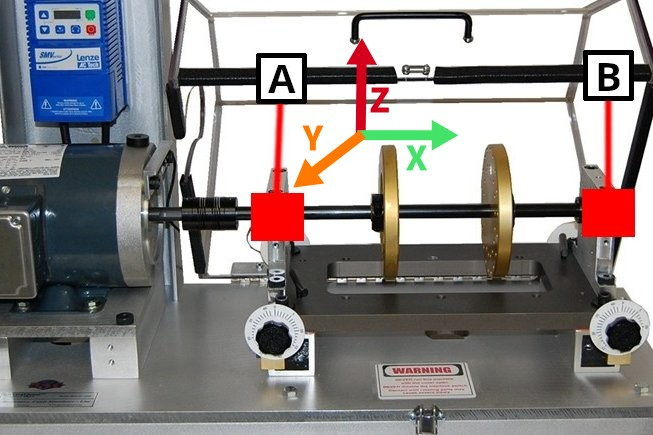
\includegraphics[width=\textwidth]{fig/sensor/mafaulda-simulator.jpg}
         \caption{MaFaulDa}
         \label{fig:mafaulda-simulator}
     \end{subfigure}
     \hfill
     \begin{subfigure}[b]{0.24\textwidth}
         \centering
         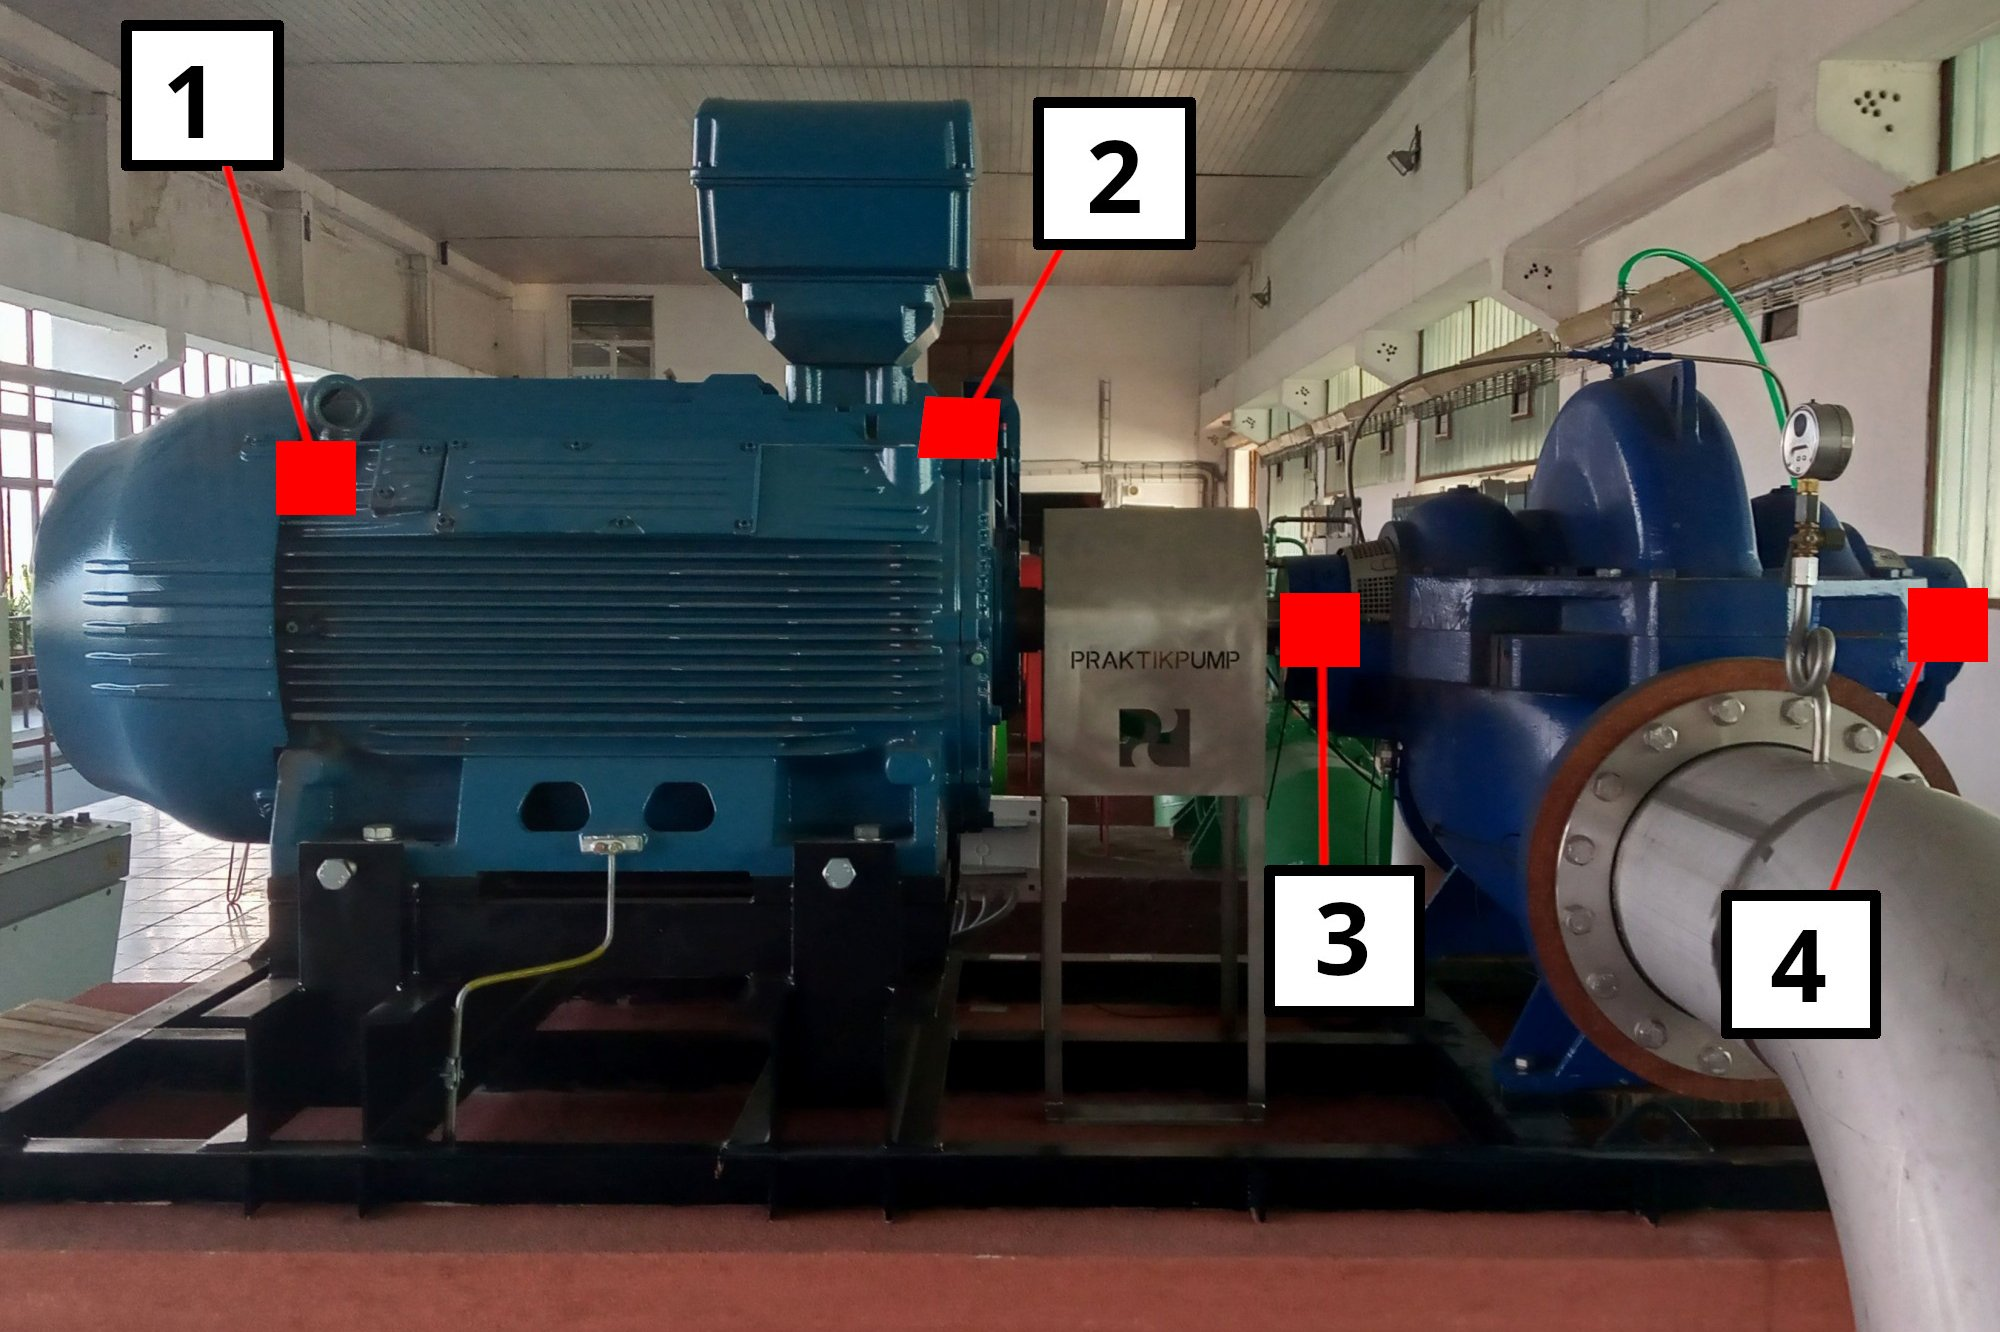
\includegraphics[width=\textwidth]{fig/sensor/ksb-pump.jpg}
         \caption{Water pump}
         \label{fig:water-pump}
     \end{subfigure}
     \hfill
     \begin{subfigure}[b]{0.24\textwidth}
         \centering
         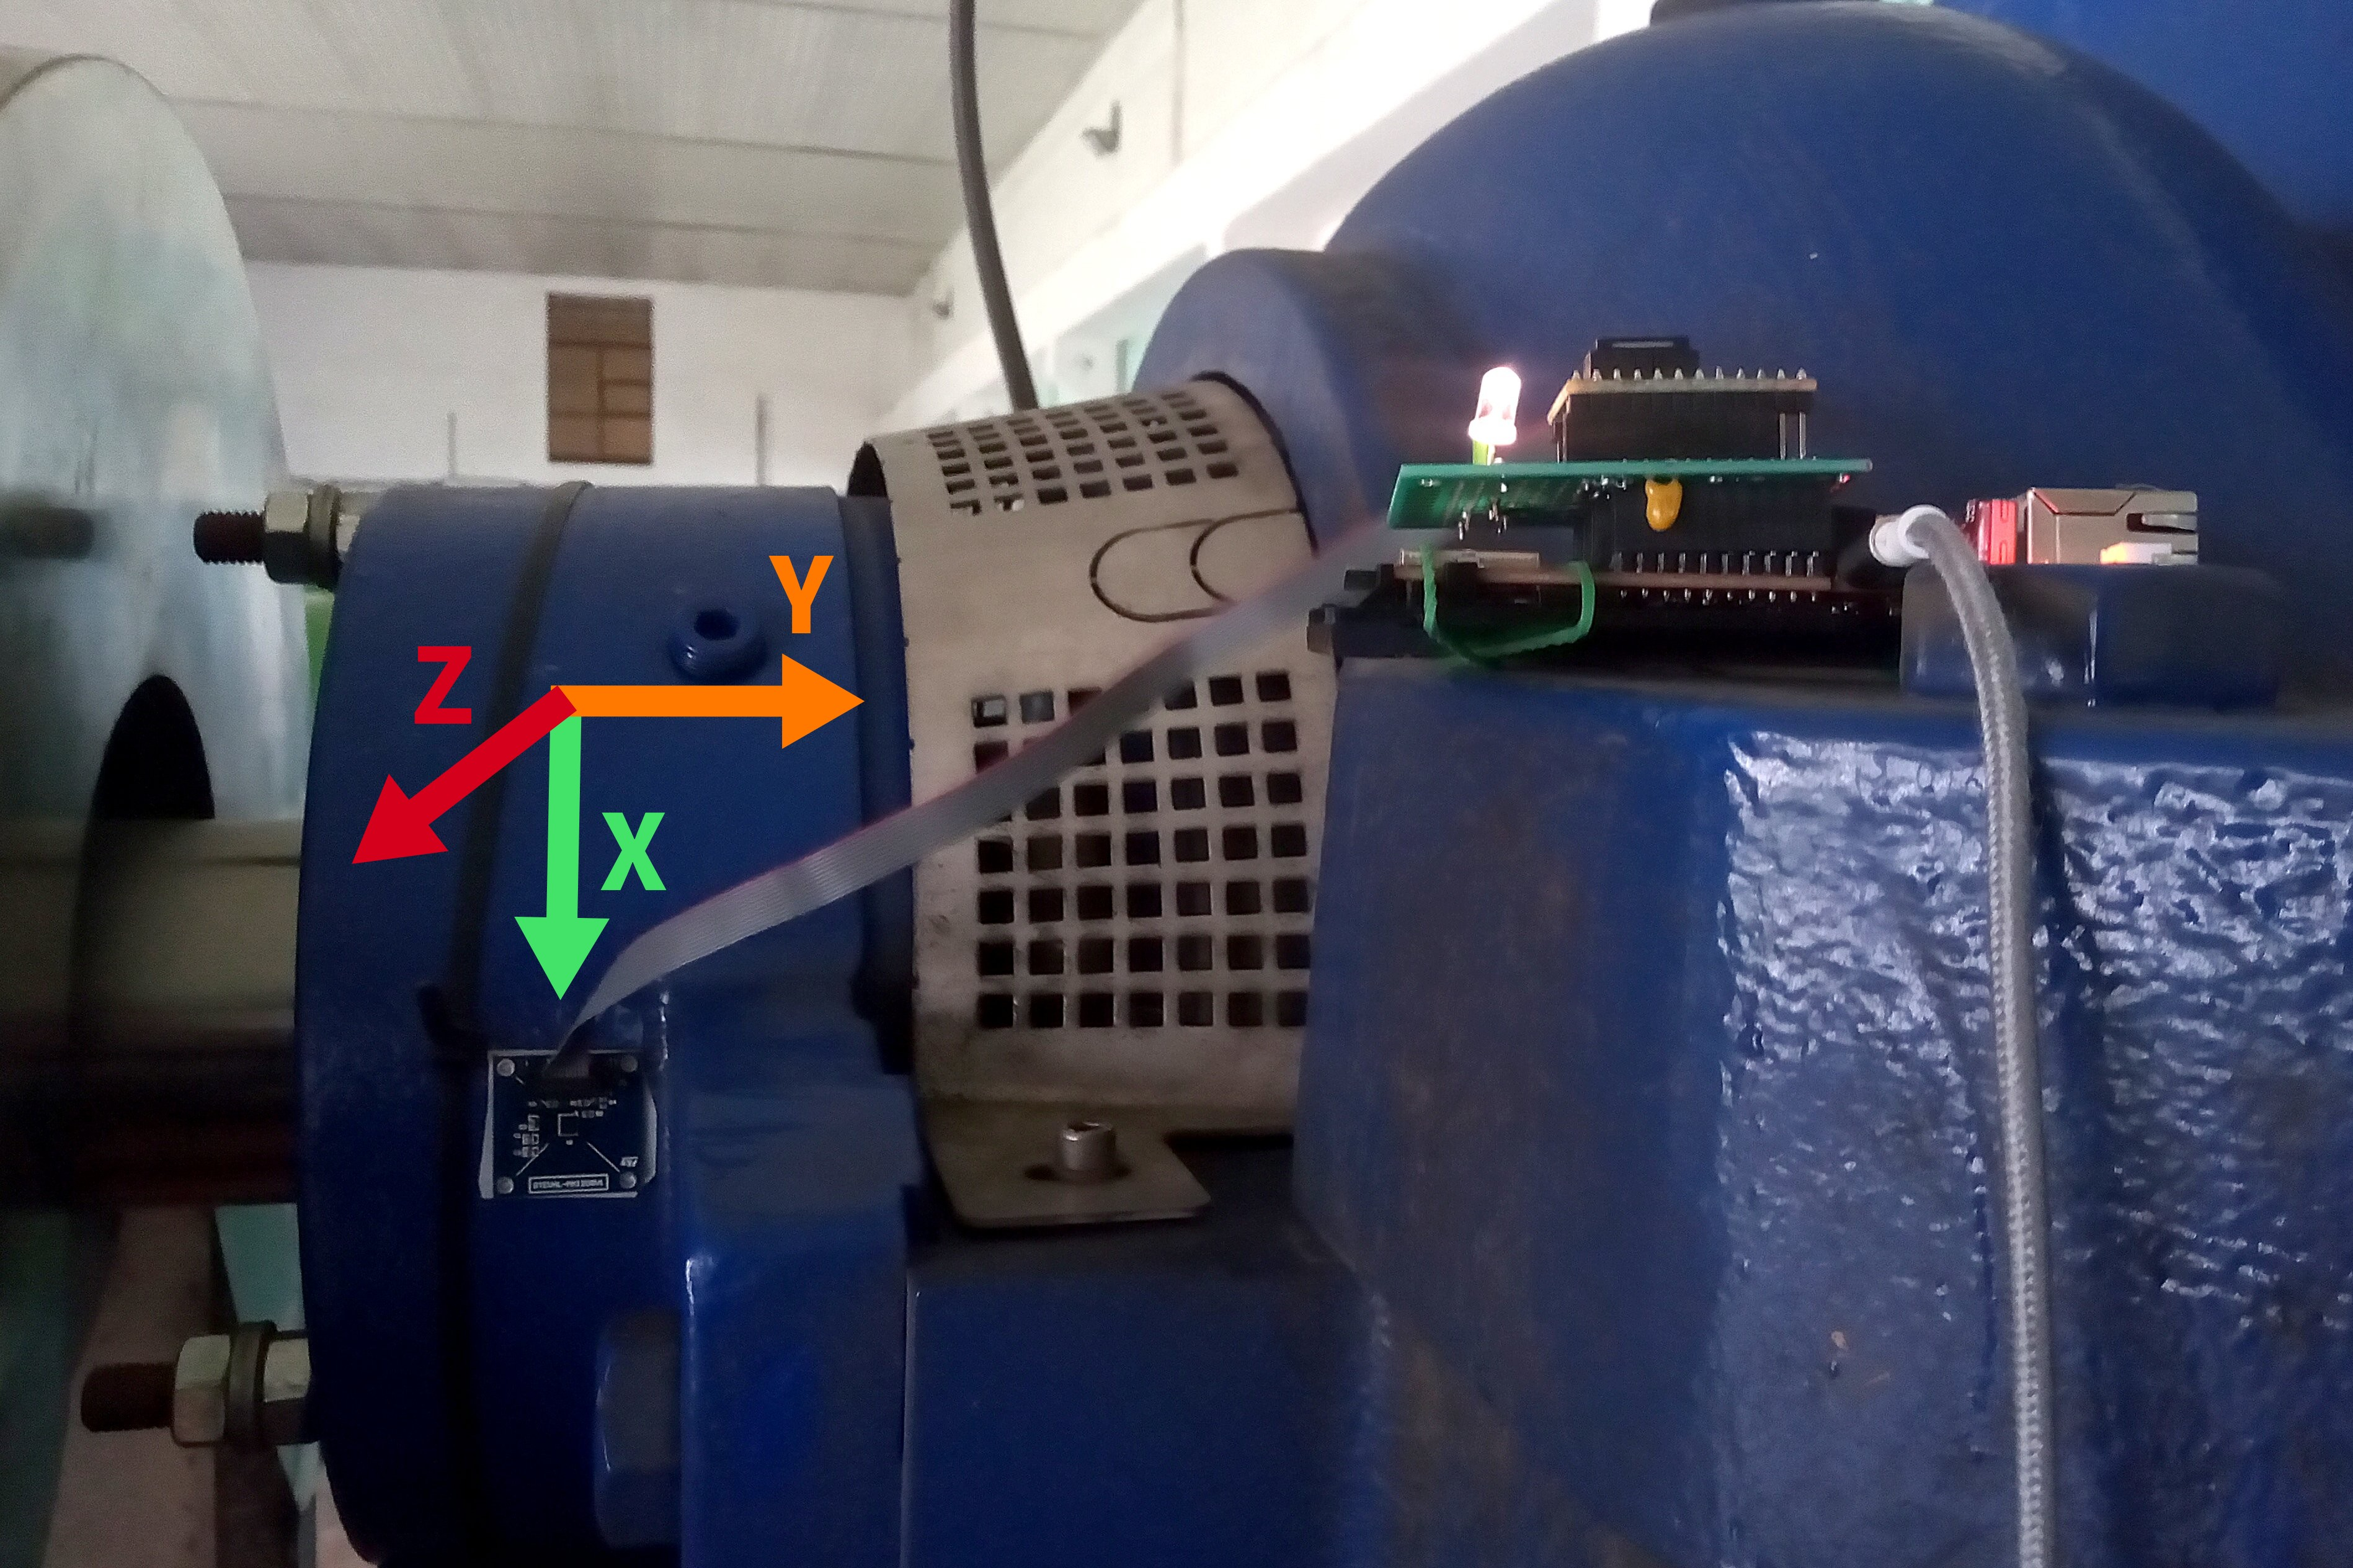
\includegraphics[width=\textwidth]{fig/sensor/sensor.jpg}
         \caption{Accelerometer}
         \label{fig:steval-sensor}
     \end{subfigure}
     \hfill
     \begin{subfigure}[b]{0.24\textwidth}
         \centering
         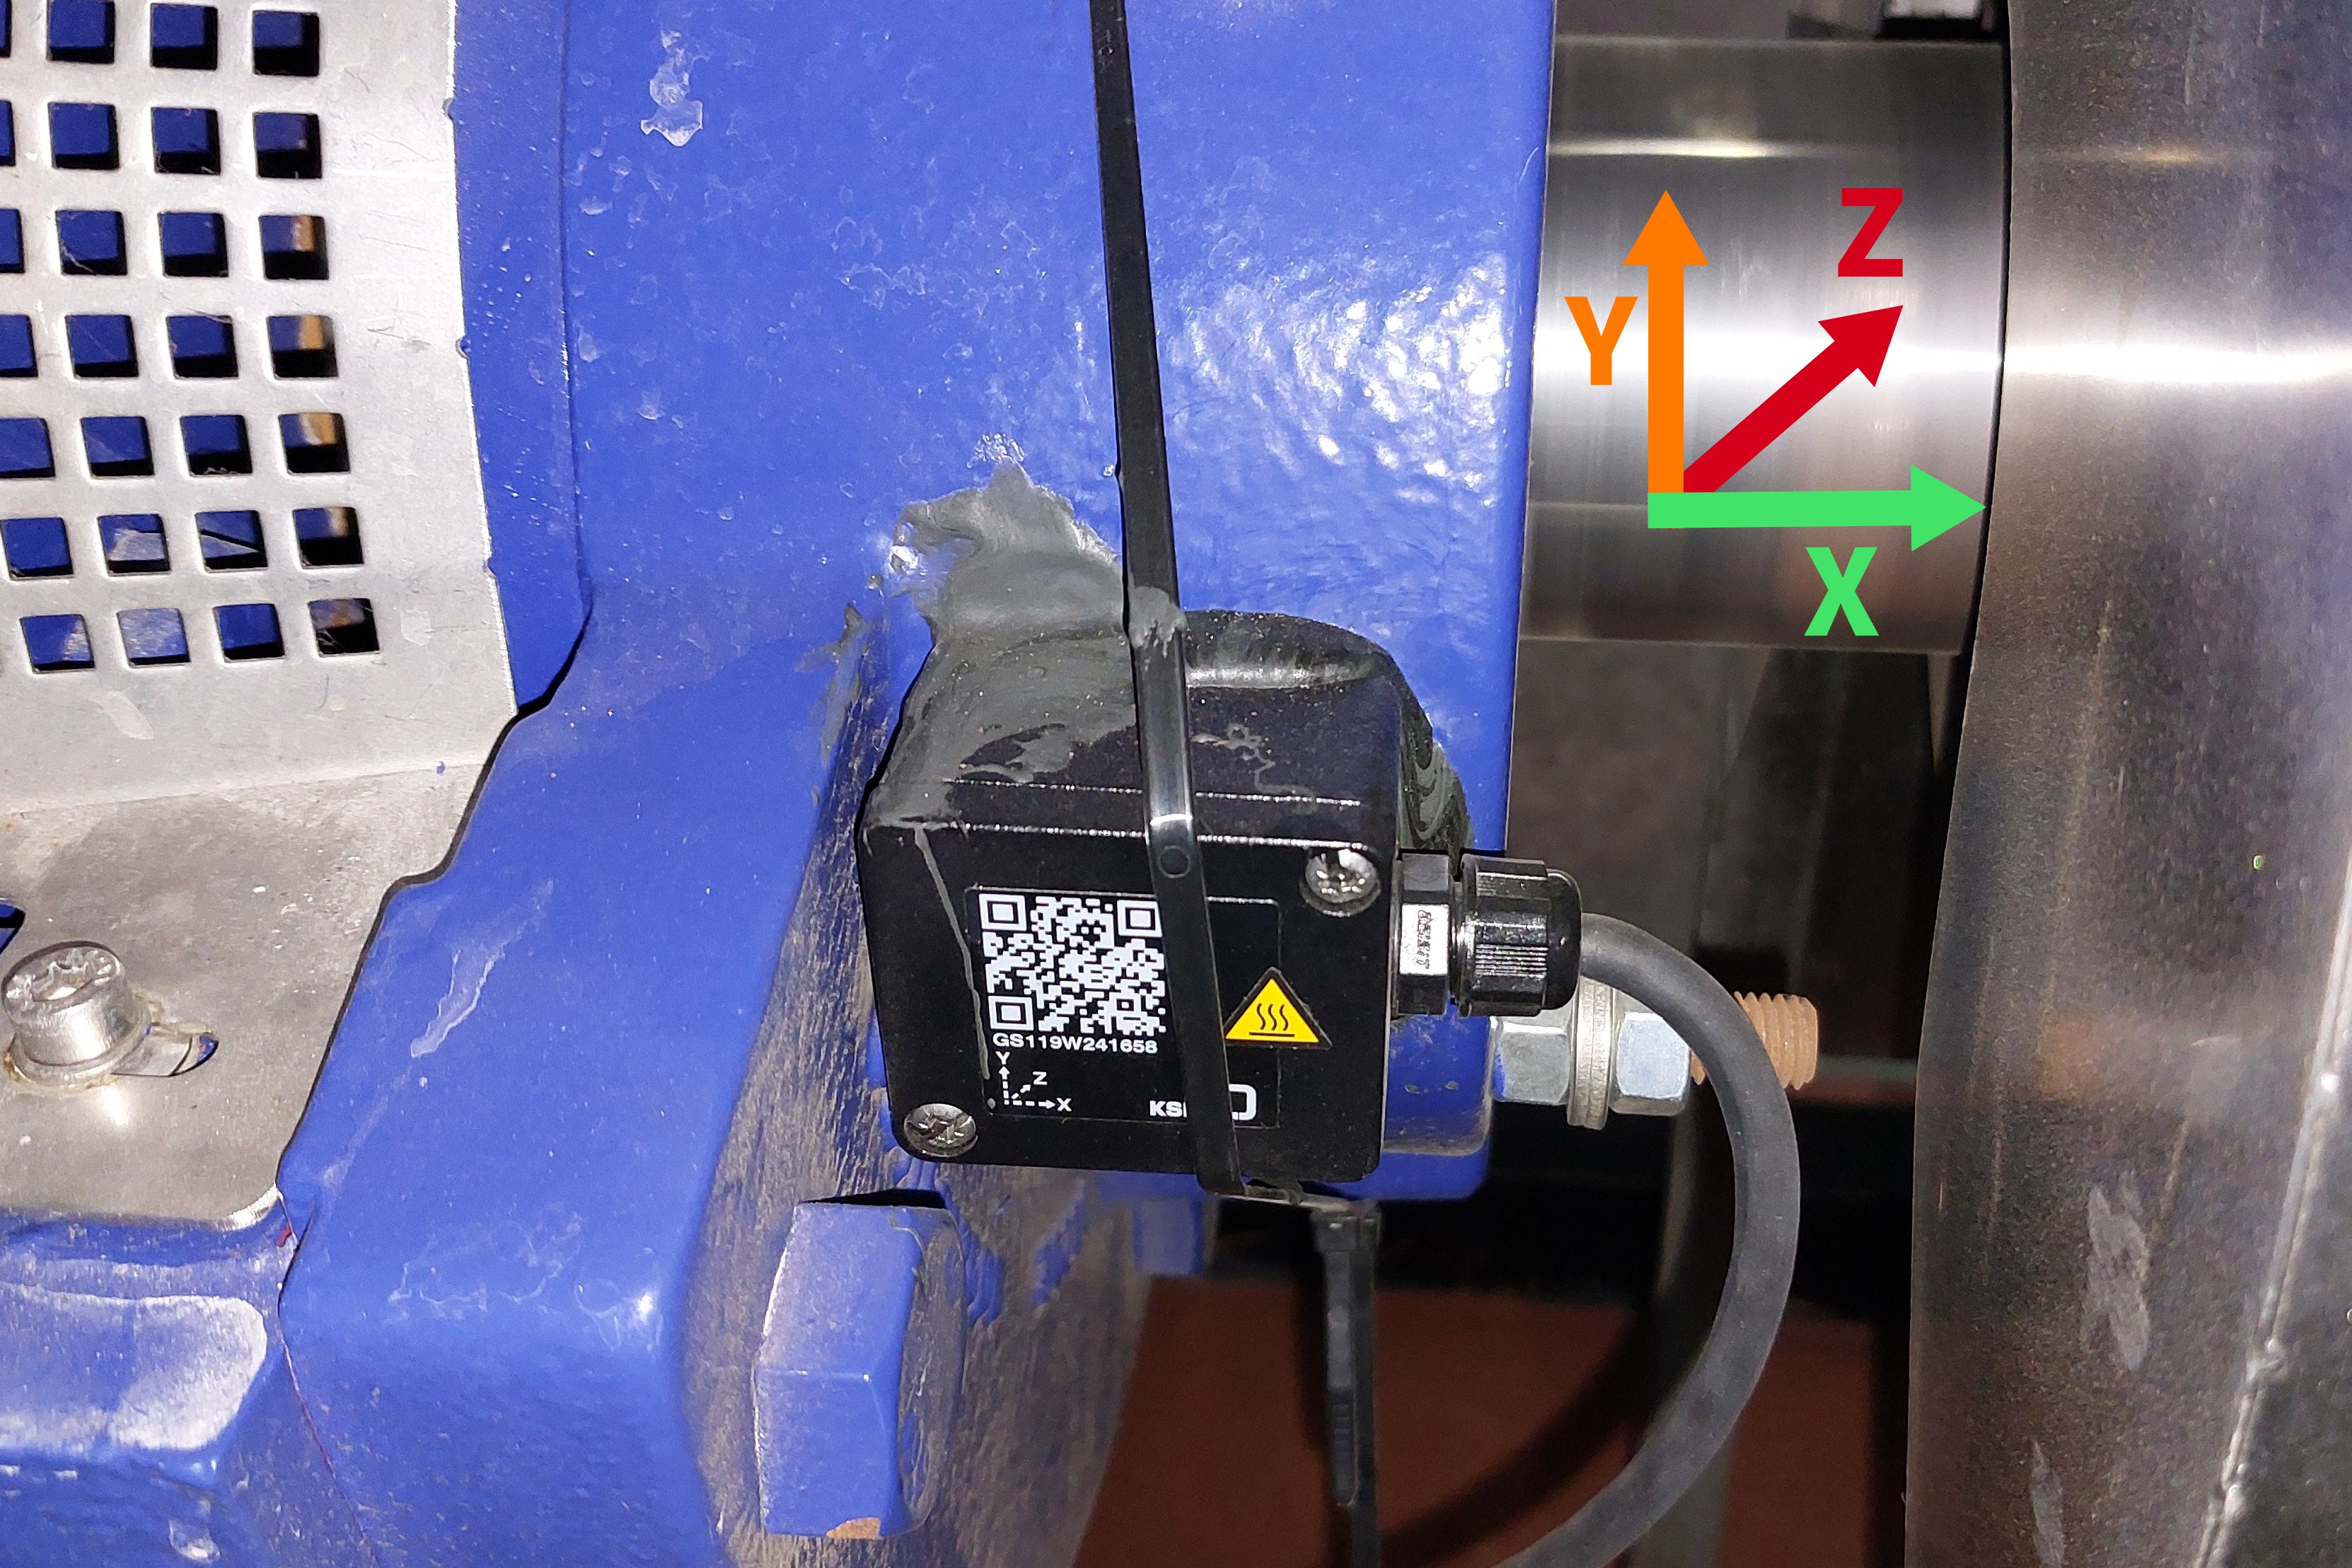
\includegraphics[width=\textwidth]{fig/sensor/ksb-cloud.jpg}
         \caption{KSB sensor}
         \label{fig:ksb-cloud-sensor}
     \end{subfigure}
     \caption{Measurement positions and accelerometer orientations}
\end{figure}

Data preprocessing of MaFaulDa is necessary to create feature sets in TD and FD. This process has several phases.
\begin{enumerate}
\item \textbf{Signal filtering}: Subtraction of overall mean removes DC component. IIR Butterworth low pass filter of 5th order attenuates frequencies above 10 kHz.
\item \textbf{Feature extraction}: Machine behavior in one time series is time-invariant. Therefore, features are calculated out of the whole duration. Frequency domain features are produced using Welch's method for power spectrums from FFT with $2^{15}$ long Hann windows and 50\% overlap  (bin resolution of 1.53~Hz). The resulting features belong to domains making up respective feature sets:
\begin{enumerate}
\item \textbf{10 features in time domain} (TD): peak-to-peak amplitude, zero-crossing rate, root mean square, skewness, kurtosis, shape factor, crest factor, impulse factor, clearance factor, average amplitude change,
\item \textbf{11 features in frequency domain} (FD): spectral centroid, standard deviation, skewness, kurtosis, roll-on frequency of 5\% total energy, roll-off frequency of 85\% total energy, spectral flux as an average correlation of separate windows, noisiness as a signal to noise ratio, spectral negentropy~\cite{avoci_spectral_2020}, energy, entropy.
\end{enumerate}
In summary 627 time domain and 1012 frequency domain feature subsets are evaluated by the same number of 5-fold cross-validated k-NN models for each value of k. 
\item \textbf{Labeling}: Three target variables are constructed out of the inner bearing, both bearings and high severity defects on both bearings. The predicted variable has 6 classes: normal, misalignment (merged vertical and horizontal), imbalance, outer race fault, ball fault, and cage fault. In the "high severity" scenario, the normal class is assigned to observations where the weight or shaft shift applied is in lower half of all of the configurations for that fault numbered from least to most severe.
\item \textbf{Class balancing}: Random oversampling strategy is used on all classes except the majority one.
\end{enumerate}

Vibrations from pumps in municipal pumping station for drinking water in Podunajské Biskupice reveal practical challenges for the deployment of machine learning models in the industry. Two pumps (P1, P2) of the same type KSB Omega 300-560, and two electric motors WEG W50 (M1, M2) were designated for measurements. Both machines have power 400~kW (ISO 20186 class~\rom{3}) and the main shaft rotates at 1493~RPM. For purposes of expert labeling, the bearing designations at numbered places are 6319-C3 (1), 6324-C3 (2), and 6317-2Z (3\&4). Sensors were placed above bearings in numbered positions according to ISO 13373 (Fig.~\ref{fig:water-pump}) with axis orientation depicted in Fig.~\ref{fig:steval-sensor}. Each pump is equipped with KSB cloud monitoring at the place (3) (Fig.~\ref{fig:ksb-cloud-sensor}) from which RMS velocity in mm/s is available for a year in hourly intervals. 

Our accelerometer ST IIS3DWB mounted to the machine using thin double-sided tape has a wideband 5 kHz linear response sampled at 26.87~kHz. Microcontroller ESP32-POE-ISO stored triaxial 60-second long recordings onto an SD card. In total 48 time series were gathered, 6 in each place. These are split into 5-second intervals for 576 data points overall. Fault labels are missing, therefore we analyze rotational speeds and defective bearing frequencies in the frequency spectrum. The observations from machines are labeled based on source machinery to 4 classes: M1, M2, P1, P2; based on sensor position to 8 classes: M1-1, M1-2, P1-3, P1-4, etc.

\section{Results}
In qualitative exploratory data analysis, representative observations from both datasets are examined through their frequency spectra in the radial direction. Patterns for categories of faults in MaFaulDa with shaft speed around 2500 RPM and in conditions of the worst severity are depicted in the wideband spectrum with a range up to 2.5 kHz (Fig.~\ref{fig:mafaulda-wideband}). Clear distinctions in spectra are apparent for different labels. The rotational frequency shows up as a spike in each case and is the only one in a normal state. Misalignment gives rise in amplitude to \nth{6} RPM harmonic, whereas imbalance excites even more harmonic frequencies.

\begin{figure}
     \begin{subfigure}[b]{0.3\textwidth}
         \centering
         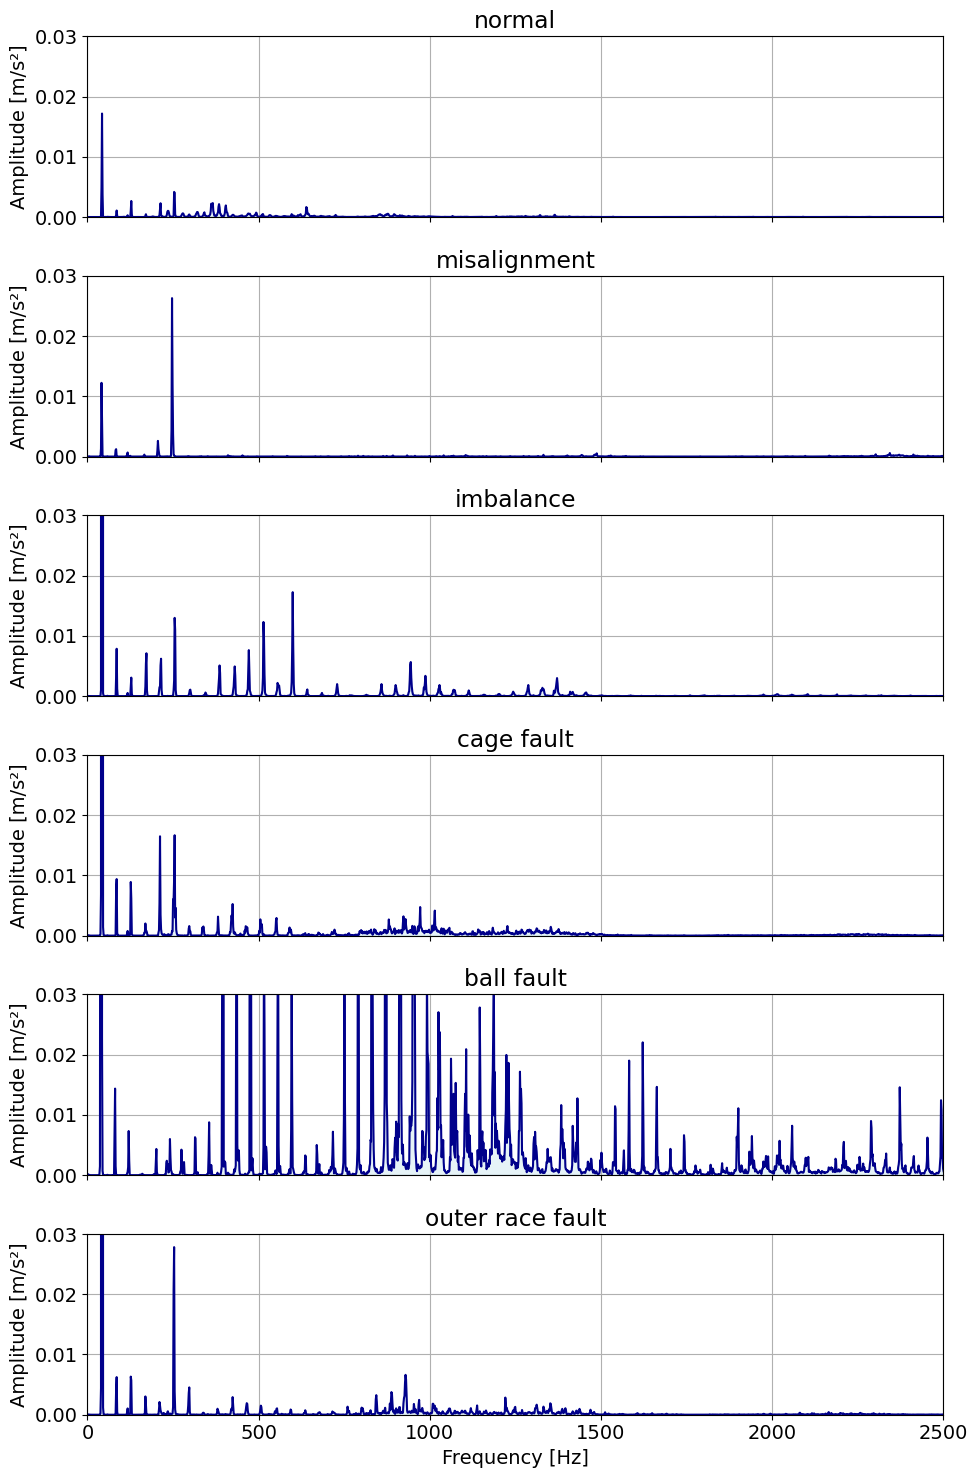
\includegraphics[width=\textwidth]{fig/spectrum/mafaulda-wideband.png}
         \caption{MaFaulDa}
         \label{fig:mafaulda-wideband}
     \end{subfigure}
     \hfill
     \begin{subfigure}[b]{0.3\textwidth}
         \centering
         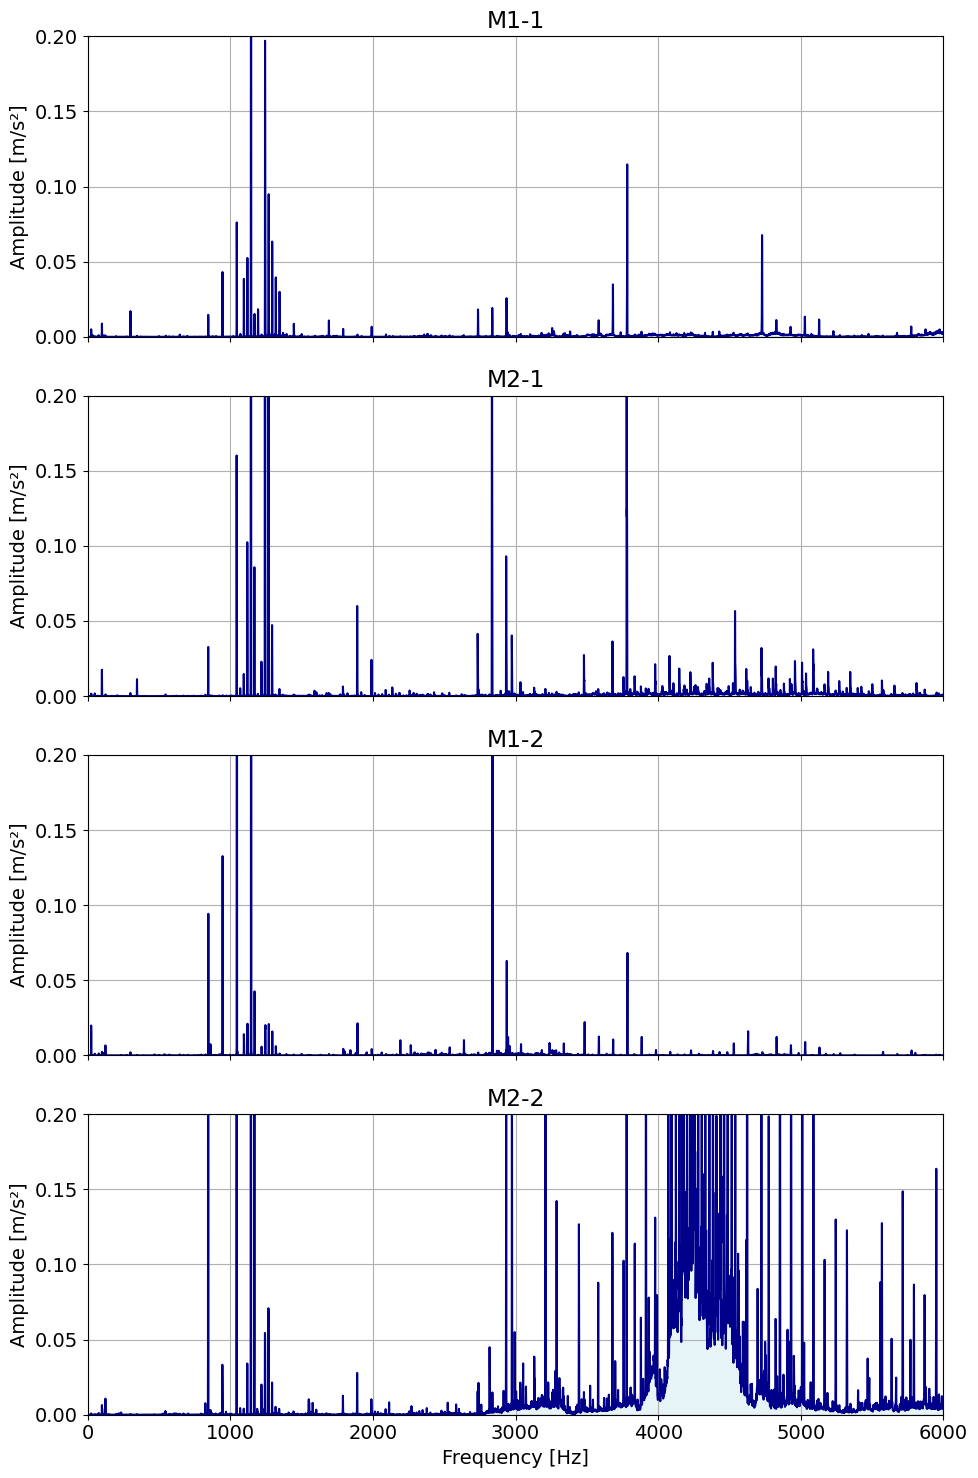
\includegraphics[width=\textwidth]{fig/spectrum/motor-wideband-60s.png}
         \caption{Motors}
         \label{fig:motor-wideband}
     \end{subfigure}
     \hfill
     \begin{subfigure}[b]{0.3\textwidth}
         \centering
         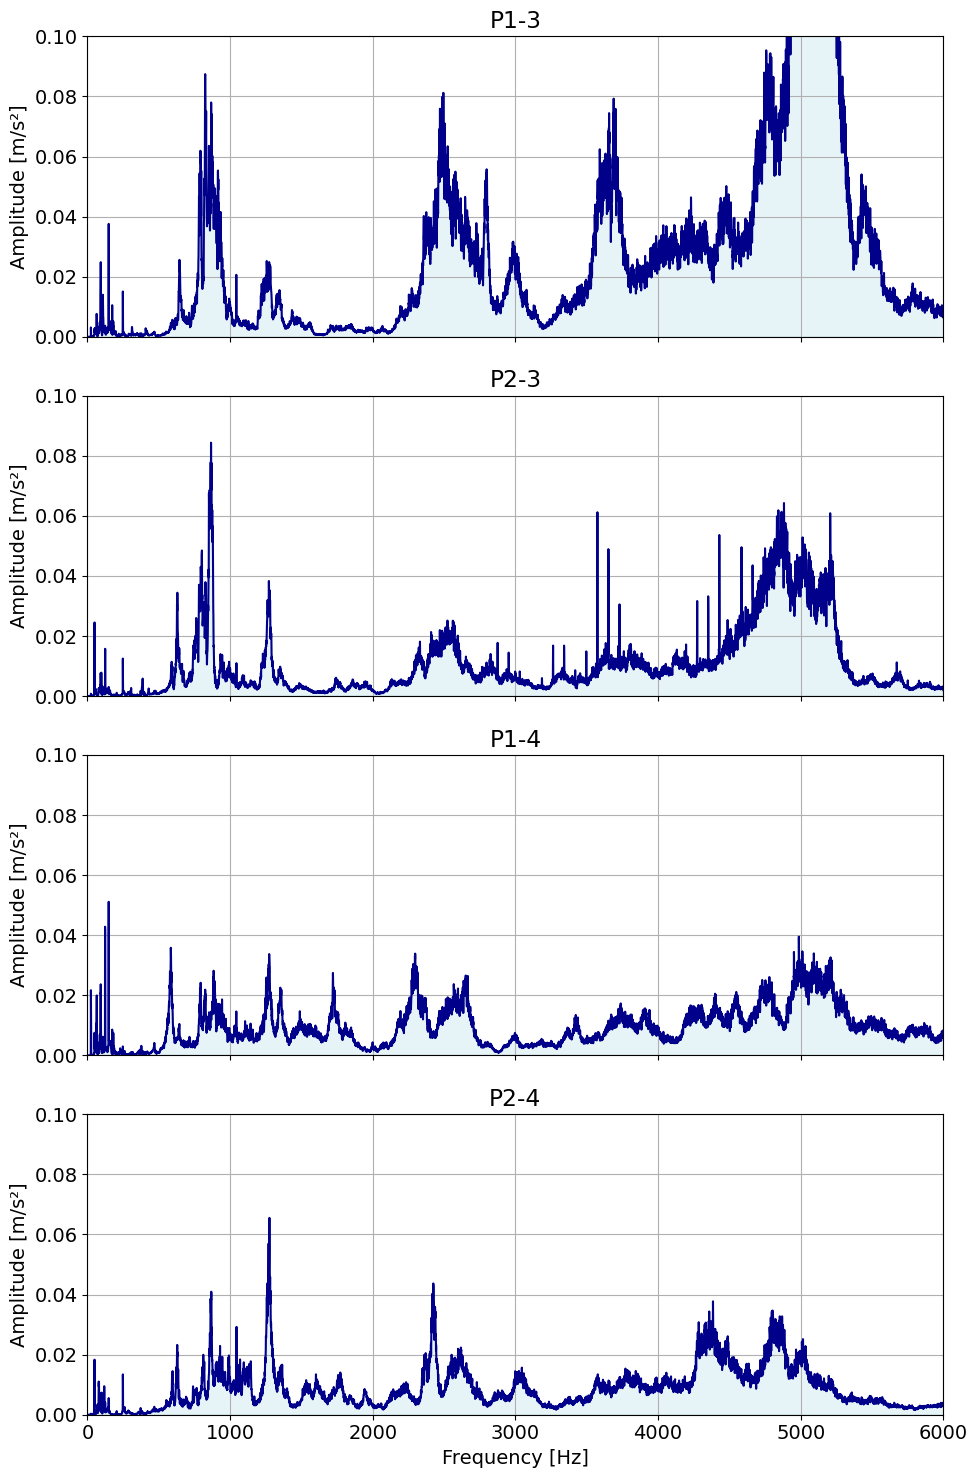
\includegraphics[width=\textwidth]{fig/spectrum/pump-wideband-60s.png}
         \caption{Pumps}
         \label{fig:pump-wideband}
     \end{subfigure}
     \caption{Wideband power spectrum}
\end{figure}

The wideband spectrum of the electric motor is polluted by the wind coming out of the back fan blades (Fig~\ref{fig:motor-wideband}). Pump spectra are lookalike in the same respective positions (Fig~\ref{fig:pump-wideband}). P1 has significantly more energy than P2 in frequency bands around 2.5 kHz, 3.6 kHz, and 5 kHz and in low frequencies. This energy can indicate a fault in the early stages because amplitudes are not tall enough. The range of amplitudes measured is at most $\pm 50$ m/$s^2$.

The long-term vendor's pump monitoring system confirms that the velocity of vibrations is still in normal conditions. Levels in radial axis (z) are almost identical for both pumps circa 1.6 mm/s (Fig.~\ref{fig:ksb-rms}).

\begin{figure}
     \begin{subfigure}[b]{0.48\textwidth}
         \centering
         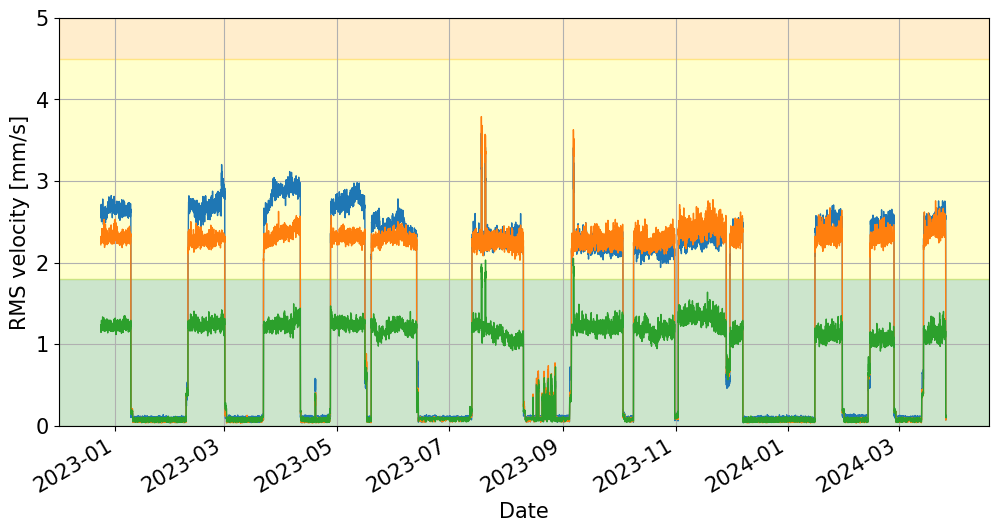
\includegraphics[width=\textwidth]{fig/ksb-cloud/P1-rms-vibration.png}
         \caption{P1-3}
         \label{fig:P1-ksb-rms}
     \end{subfigure}
     \hfill
     \begin{subfigure}[b]{0.48\textwidth}
         \centering
         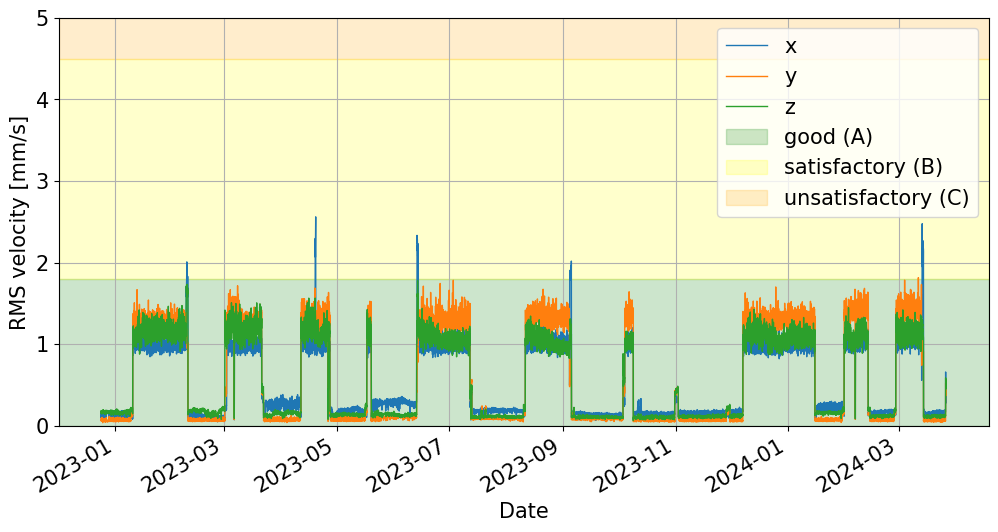
\includegraphics[width=\textwidth]{fig/ksb-cloud/P2-rms-vibration.png}
         \caption{P2-3}
         \label{fig:P2-ksb-rms}
     \end{subfigure}
     \caption{Vibrations of water pumps and ISO severity levels}
     \label{fig:ksb-rms}
\end{figure}

\begin{table}
\centering
\caption{Numbers of observations by label in MaFaulDa}
\label{tab:mafaulda-observation-counts}
\begin{tabular}{|l|r|r|r|}
\hline
\textbf{Label} &  \textbf{Bearing A} & \textbf{Both bearings} & \textbf{Severity} \\
\hline
normal            &  49  &  49  &  1125 \\
misalignment      & 498  &  498 & 198 \\
imbalance         & 333  &  333 & 139 \\
cage fault        & 188  &  376 & 181 \\
ball fault        & 186  &  323 & 132 \\
outer race fault  & 184  &  372 & 176 \\
\hline
$\Sigma$ & 1438  & 1951 & 1951 \\
\hline
\end{tabular}
\end{table}

Scatter plots (Fig.~\ref{fig:mafaulda-scatter}, \ref{fig:pump-scatter}) visualize the spatial distribution of labels for entire feature sets after min-max scaler and PCA. Explained variance percentages are next to the component's name. Labels are assigned in three different ways producing observation counts according to Table~\ref{tab:mafaulda-observation-counts}. The imbalance ratio in the MaFaulDa dataset is 1016\% for original classes and 852\% for high-severity modification. Colored regions are decision boundaries of the k-NN classifier trained on 80\% of the PCA transformed dataset. 

Misalignment and ball fault groups are separated the best from the rest but the imbalance group is intertwined with bearing faults. Silhouette scores of the feature sets of the MaFaulDa after min-max scaling are 0.05 (TD) and 0.14 (FD). Sensor placements on pumps have silhouette scores of 0.20 (TD) and 0.21 (FD).


\begin{figure}
	\centering
     \begin{subfigure}[b]{0.24\textwidth}
         \centering
         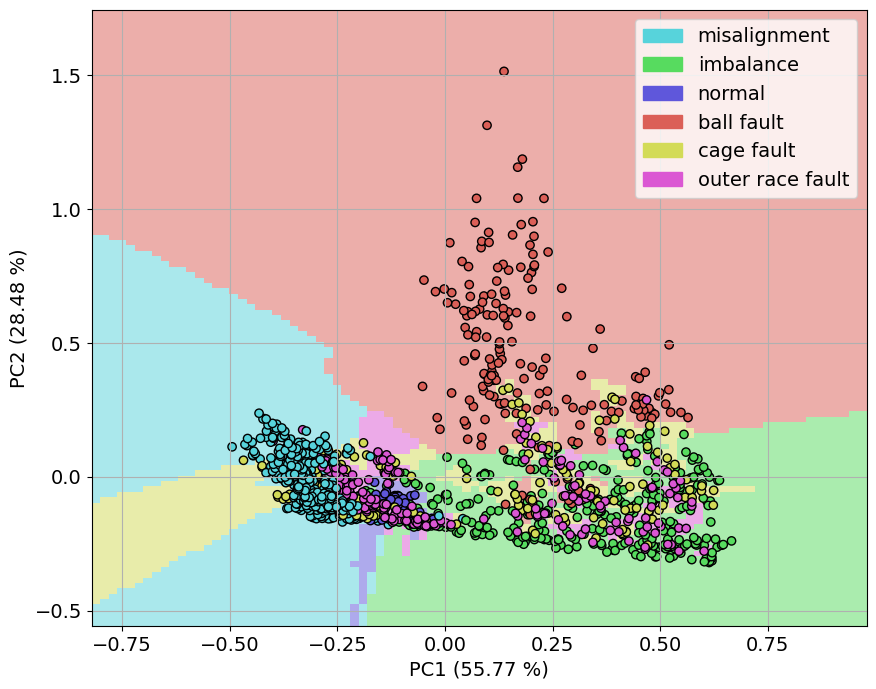
\includegraphics[width=\textwidth]{fig/scatter-mafaulda/td-a-bearing.png}
         \caption{Bearing A in TD}
     \end{subfigure}
     \hfill
     \begin{subfigure}[b]{0.24\textwidth}
         \centering
         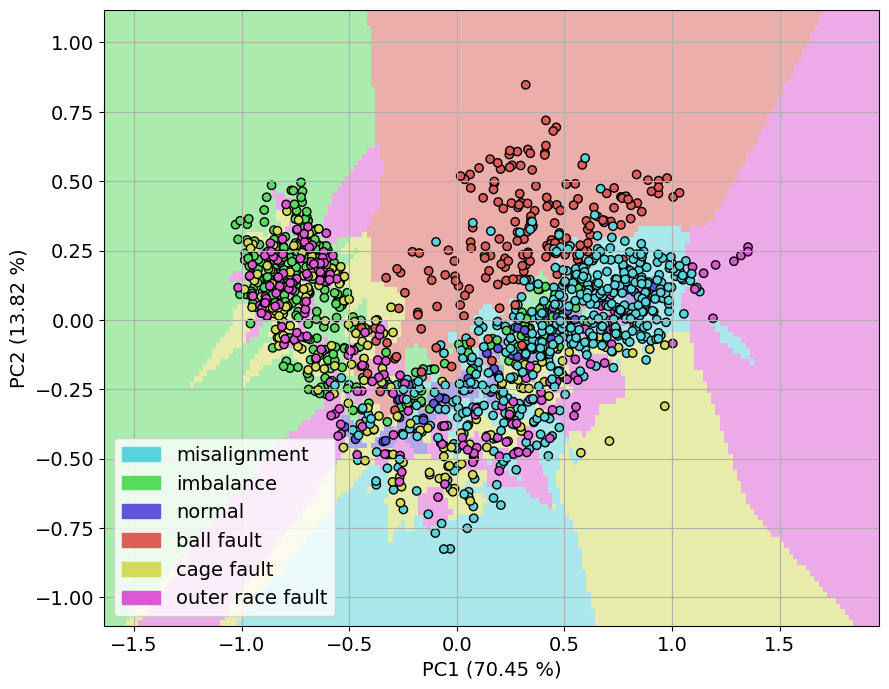
\includegraphics[width=\textwidth]{fig/scatter-mafaulda/fd-a-bearing.png}
         \caption{Bearing A in FD}
     \end{subfigure}
     \hfill
     \begin{subfigure}[b]{0.24\textwidth}
         \centering
         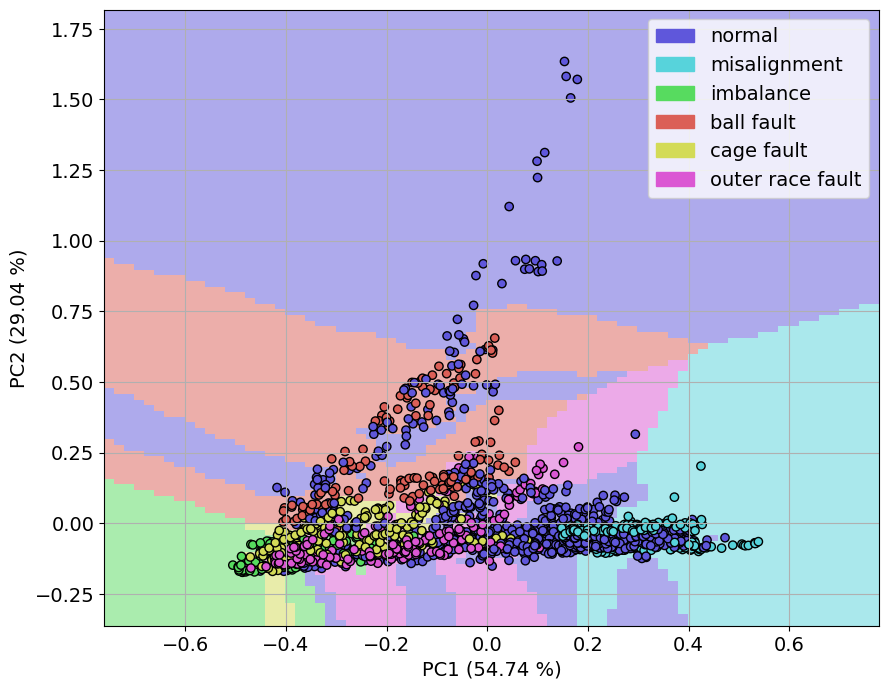
\includegraphics[width=\textwidth]{fig/scatter-mafaulda/td-severity.png}
         \caption{Severity in TD}
     \end{subfigure}
     \hfill
     \begin{subfigure}[b]{0.24\textwidth}
         \centering
         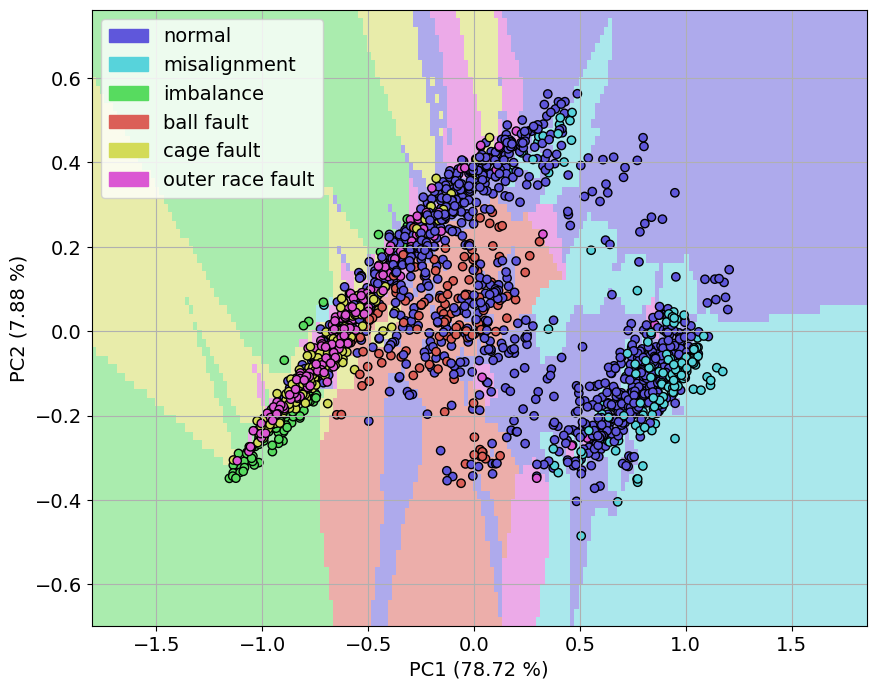
\includegraphics[width=\textwidth]{fig/scatter-mafaulda/fd-severity.png}
         \caption{Severity in FD}
     \end{subfigure}
     \caption{PCA scatter plots of MaFaulDa with 5-NN decision boundaries}
     \label{fig:mafaulda-scatter}
\end{figure}

\begin{figure}[h]
	\centering
     \begin{subfigure}[b]{0.24\textwidth}
         \centering
         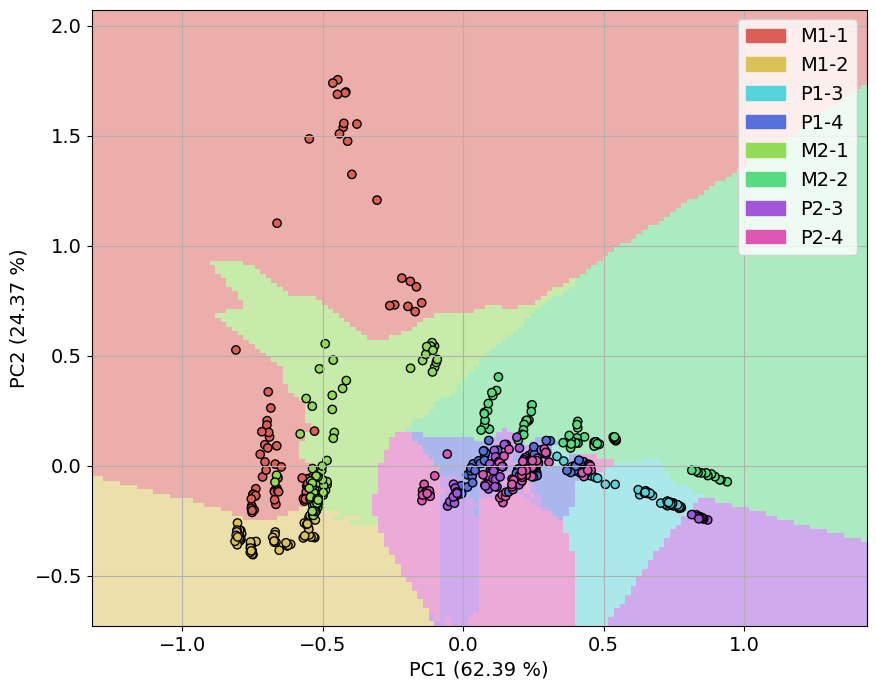
\includegraphics[width=\textwidth]{fig/scatter-pumps/position-td.png}
         \caption{Positions in TD}
     \end{subfigure}
     \hfill
     \begin{subfigure}[b]{0.24\textwidth}
         \centering
         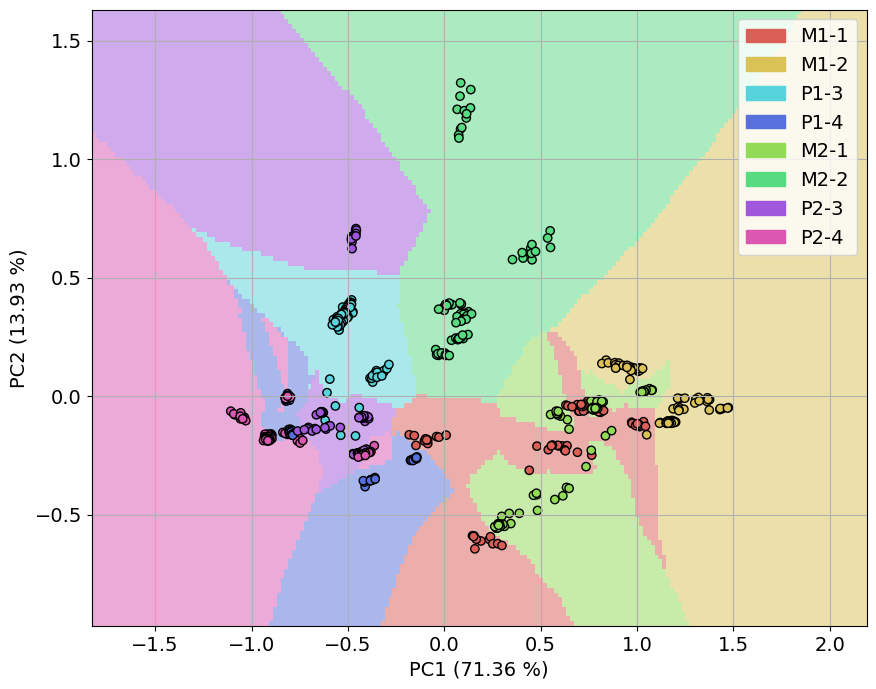
\includegraphics[width=\textwidth]{fig/scatter-pumps/position-fd.png}
         \caption{Positions in FD}
     \end{subfigure}
     \hfill
     \begin{subfigure}[b]{0.24\textwidth}
         \centering
         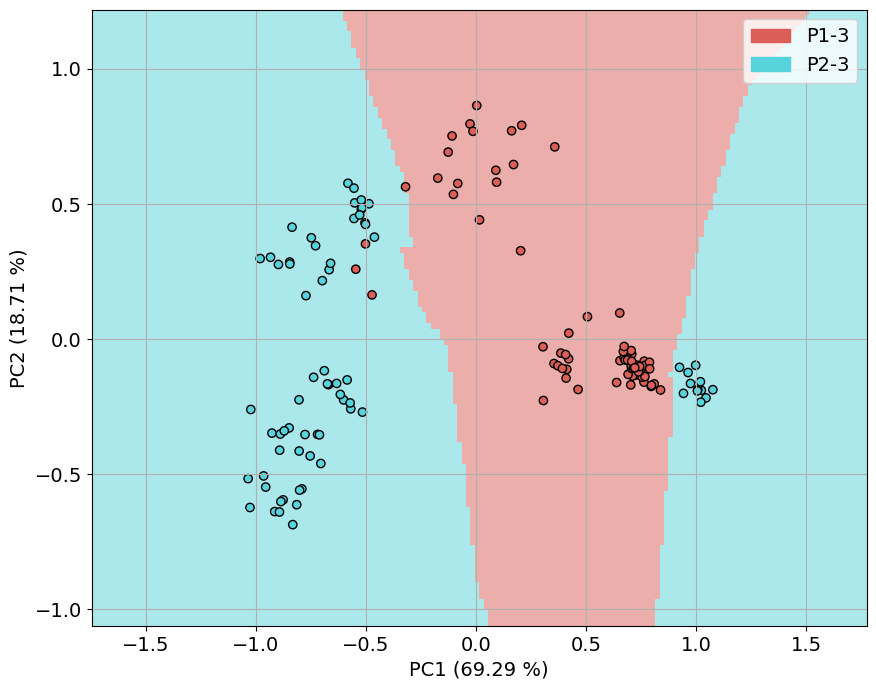
\includegraphics[width=\textwidth]{fig/scatter-pumps/binary-td.png}
         \caption{P1-3/P2-3 in TD}
     \end{subfigure}
     \hfill
     \begin{subfigure}[b]{0.24\textwidth}
         \centering
         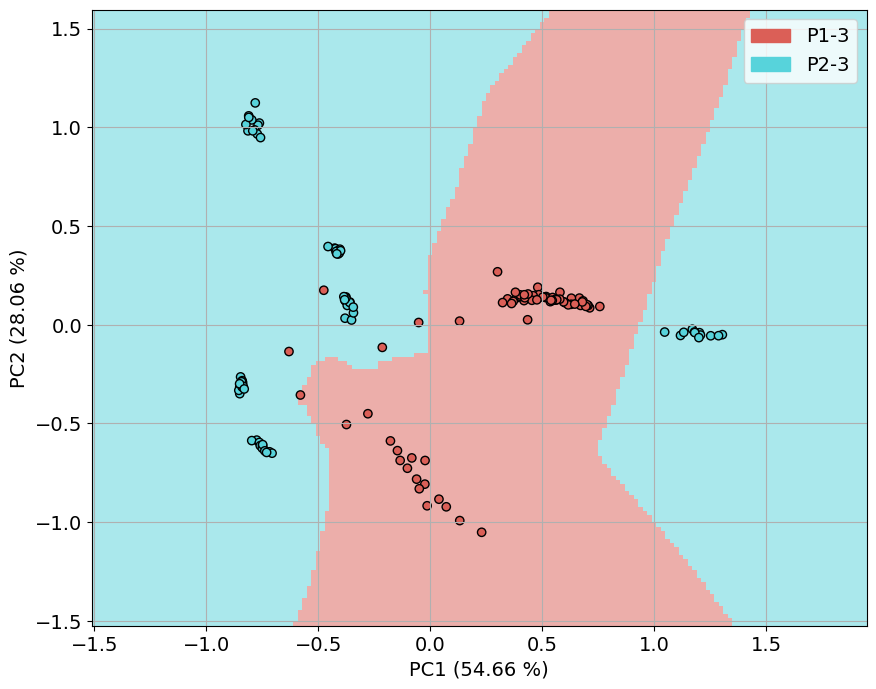
\includegraphics[width=\textwidth]{fig/scatter-pumps/binary-fd.png}
         \caption{P1-3/P2-3 in FD}
     \end{subfigure}
     \caption{PCA scatter plots of pumps with 5-NN decision boundaries}
     \label{fig:pump-scatter}
\end{figure}

The increase in hyperparameter of k for whole feature sets results in less accuracy of k-NN (Fig.~\ref{fig:accuracy-all-features}). The sharp decline of more than 10\% in some cases is noticeable for k between 1 and 9. The features extracted in the time domain have overall better accuracy than those in the frequency domain. The attributes combined from all sensor directions also reach better accuracies than just from a single axis.

\begin{figure}
	% One axis
	\centering
     \begin{subfigure}[b]{0.32\textwidth}
         \centering
         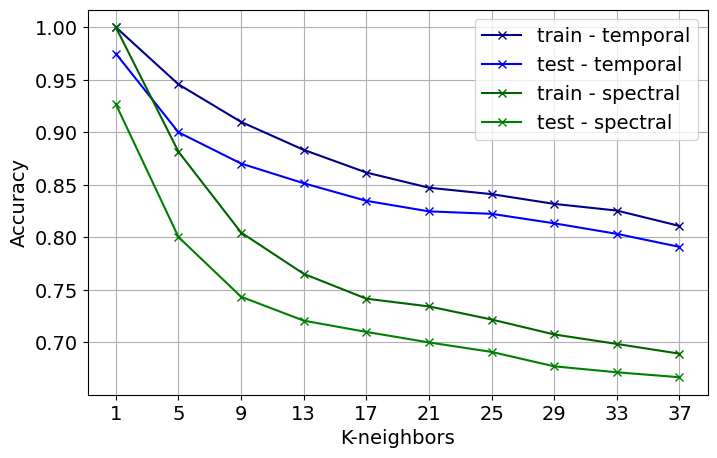
\includegraphics[width=\textwidth]{fig/all-features-mafaulda/one-axis-a-bearing.png}
         \caption{One axis, Bearing A}
     \end{subfigure}
     \hfill
     \begin{subfigure}[b]{0.32\textwidth}
         \centering
         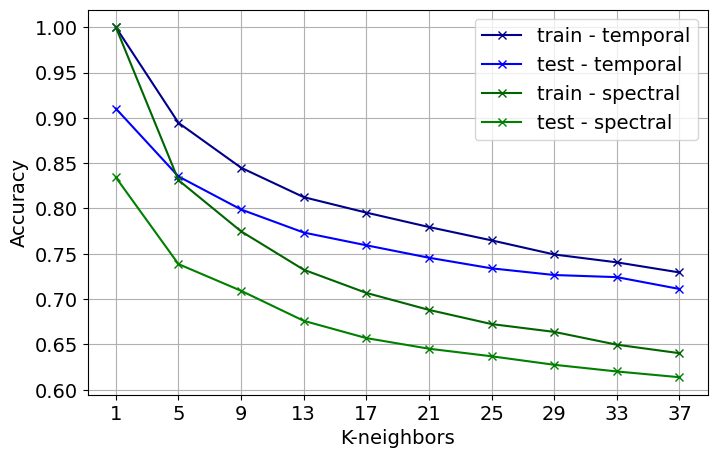
\includegraphics[width=\textwidth]{fig/all-features-mafaulda/one-axis-all-bearings.png}
         \caption{One axis, Both bearings}
     \end{subfigure}
     \hfill
     \begin{subfigure}[b]{0.32\textwidth}
         \centering
         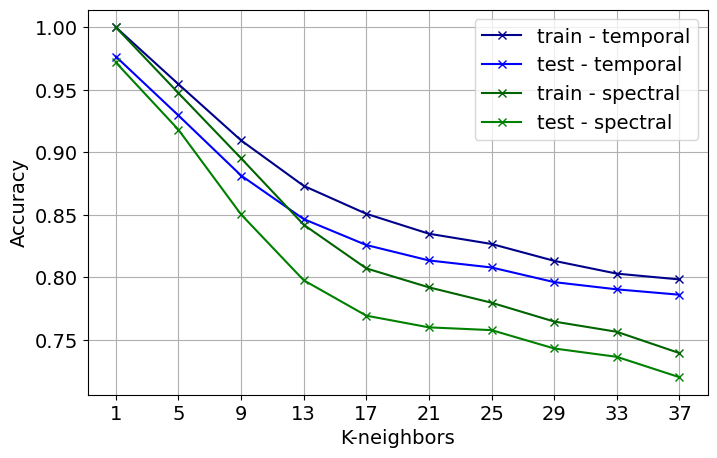
\includegraphics[width=\textwidth]{fig/all-features-mafaulda/one-axis-severity.png}
         \caption{One axis, High severity}
     \end{subfigure}
     \hfill
     % All axis
     \begin{subfigure}[b]{0.32\textwidth}
         \centering
         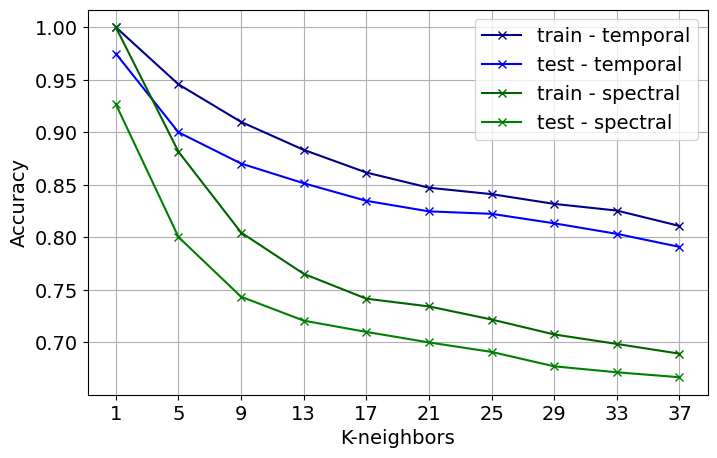
\includegraphics[width=\textwidth]{fig/all-features-mafaulda/all-axis-a-bearing.png}
         \caption{All axis, Bearing A}
     \end{subfigure}
     \hfill
     \begin{subfigure}[b]{0.32\textwidth}
         \centering
         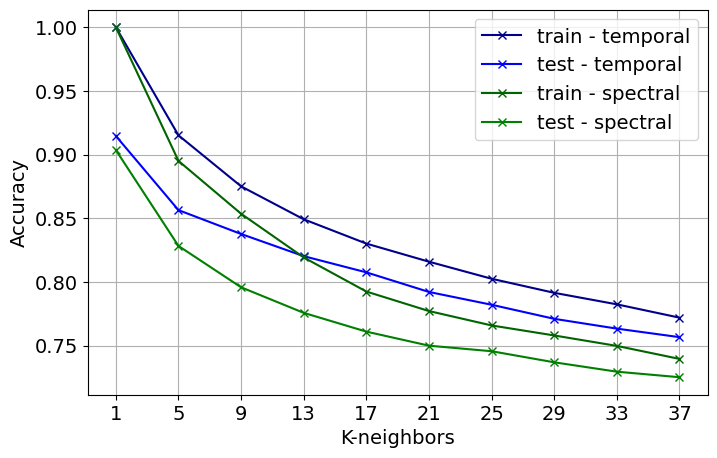
\includegraphics[width=\textwidth]{fig/all-features-mafaulda/all-axis-all-bearings.png}
         \caption{All axis, Both bearings}
     \end{subfigure}
     \hfill
     \begin{subfigure}[b]{0.32\textwidth}
         \centering
         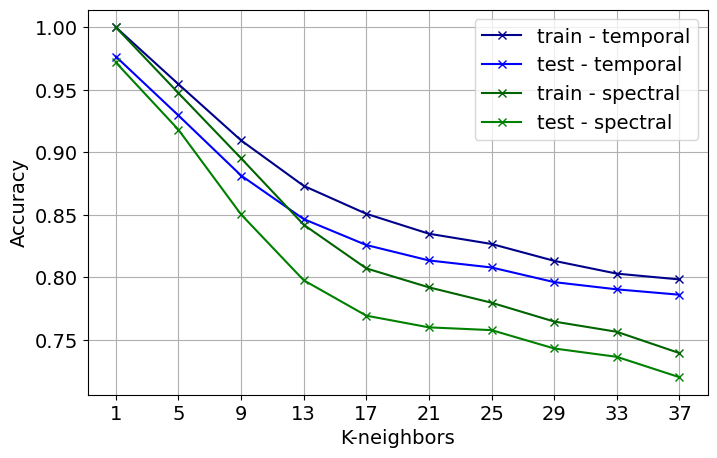
\includegraphics[width=\textwidth]{fig/all-features-mafaulda/all-axis-severity.png}
         \caption{All axis, High severity}
     \end{subfigure}
     \caption{Accuracy on MaFaulDa feature sets TD and FD depending on k value}
     \label{fig:accuracy-all-features}
\end{figure}

The tendency of decrease in accuracy with an increase in number of neighbors holds even in feature subsets (Fig.~\ref{fig:all-models-bearings-f-3}, \ref{fig:all-models-severity-f-3}). The k-NN trained with any 3 features from FD have accuracy distribution shifted higher than TD, contrary to whole feature sets. Picking a model with $k < 15$ at random always guarantees better than chance accuracy. Increasing the number of features increases the k-NN accuracies for both domains and scenarios at any k value (Fig.~\ref{fig:all-models-bearings-k-5}, \ref{fig:all-models-severity-k-5}).

\begin{figure}
	\centering
     \begin{subfigure}[b]{0.45\textwidth}
         \centering
         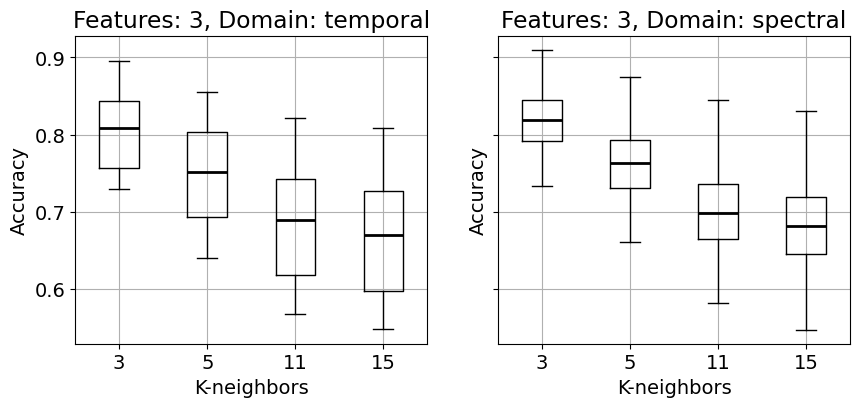
\includegraphics[width=\textwidth]{fig/combinations-mafaulda/all-axis-a-bearing-f3.png}
         \caption{Bearing A}
         \label{fig:all-models-bearings-f-3}
     \end{subfigure}
     \hfill
     \begin{subfigure}[b]{0.45\textwidth}
         \centering
         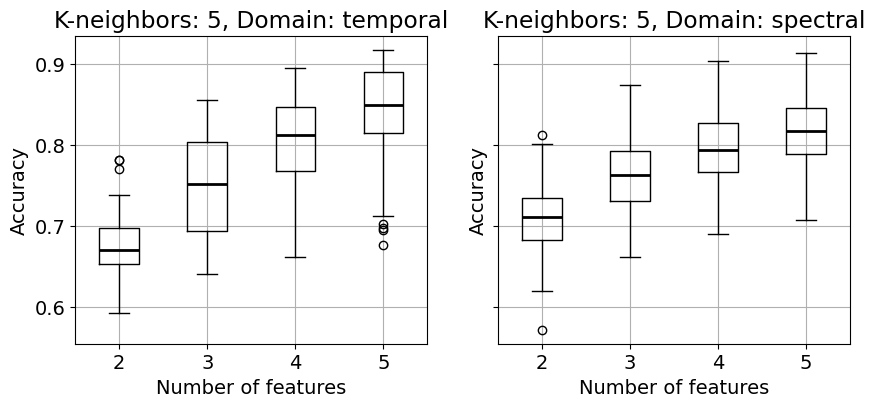
\includegraphics[width=\textwidth]{fig/combinations-mafaulda/all-axis-a-bearing-k5.png}
         \caption{Bearing A}
         \label{fig:all-models-bearings-k-5}
     \end{subfigure}
     \hfill
     \begin{subfigure}[b]{0.45\textwidth}
         \centering
         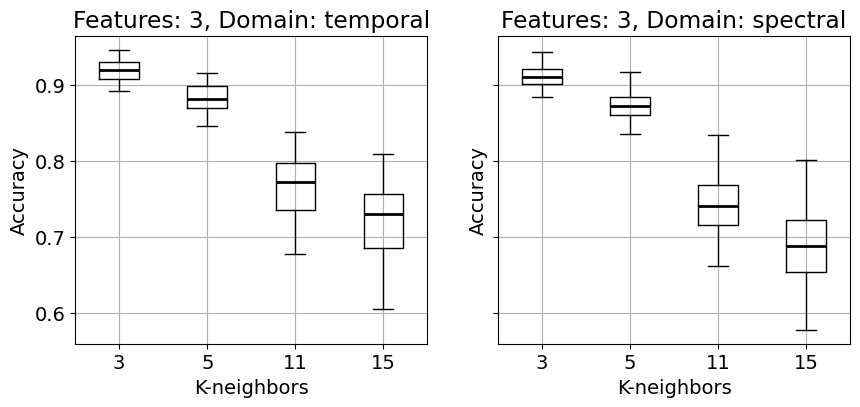
\includegraphics[width=\textwidth]{fig/combinations-mafaulda/all-axis-severity-f3.png}
         \caption{High severity}
         \label{fig:all-models-severity-f-3}
     \end{subfigure}
     \hfill
     \begin{subfigure}[b]{0.45\textwidth}
         \centering
         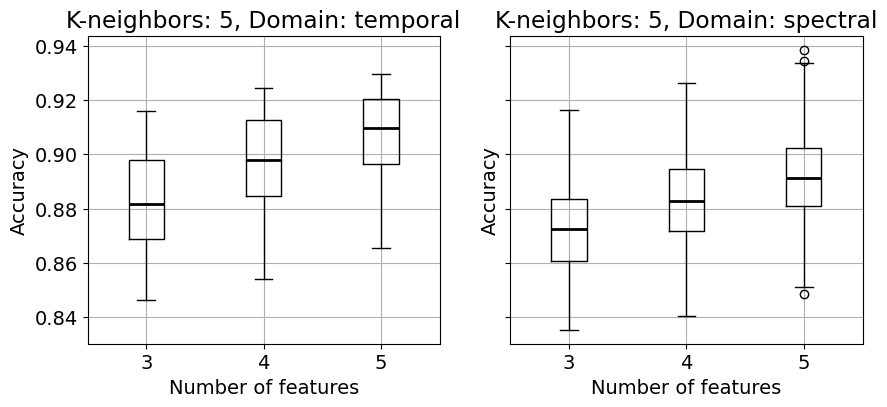
\includegraphics[width=\textwidth]{fig/combinations-mafaulda/all-axis-severity-k5.png}
         \caption{High severity}
         \label{fig:all-models-severity-k-5}
     \end{subfigure}
     \caption{Test accuracies of all combinations of feature subsets}
\end{figure}

Tables~\ref{tab:fsel-methods-td} and \ref{tab:fsel-methods-fd} compare the average 5-fold test accuracy of different feature selection methods for the k-NN model with k = 5. Three-axis features reach better accuracy the one-axis ones.

\begin{table}
\centering
\caption{Accuracy of k-NN in TD feature set and subsets of 3}
\label{tab:fsel-methods-td}
\begin{tabular}{|r|l|p{1.2cm}|p{1.2cm}|p{1.2cm}|p{1.2cm}|p{1.2cm}|p{1.2cm}|}
\hline
\multicolumn{1}{|l|}{\multirow{2}{*}{\textbf{Axis}}} & \multicolumn{1}{l|}{\multirow{2}{*}{\textbf{Method}}} & \multicolumn{2}{l|}{\textbf{Bearing A}}                                  & \multicolumn{2}{l|}{\textbf{Both Bearings}}                              & \multicolumn{2}{l|}{\textbf{High severity}}                              \\ \cline{3-8} 
\multicolumn{1}{|l|}{}                               & \multicolumn{1}{l|}{}                                 & \multicolumn{1}{l|}{\textbf{Train}} & \multicolumn{1}{l|}{\textbf{Test}} & \multicolumn{1}{l|}{\textbf{Train}} & \multicolumn{1}{l|}{\textbf{Test}} & \multicolumn{1}{l|}{\textbf{Train}} & \multicolumn{1}{l|}{\textbf{Test}} \\ \hline
\multirow{7}{*}{1}                                   & All features                                          & \textit{94.56}                      & 89.99                              & \textit{89.45}                      & 83.53                              & \textit{94.93}                      & 91.60                              \\
                                                     & PCA 3 PC                                              & \textit{88.63}                      & 80.09                              & \textit{82.87}                      & 73.66                              & \textit{92.17}                      & 87.22                              \\
                                                     & Best 3 features                                       & \textit{91.98}                      & 85.37                              & \textit{85.56}                      & 78.48                              & \textit{93.90}                      & 89.64                              \\
                                                     & Rank product                                          & \textit{87.96}                      & 79.99                              & \textit{80.71}                      & 71.42                              & \textit{93.07}                      & 88.50                              \\
                                                     & Correlation                                           & \textit{88.83}                      & 80.99                              & \textit{81.40}                      & 72.83                              & \textit{93.07}                      & 88.50                              \\
                                                     & F-statistic                                           & \textit{87.53}                      & 79.08                              & \textit{80.71}                      & 71.42                              & \textit{93.07}                      & 88.50                              \\
                                                     & Mutual information                                    & \textit{87.06}                      & 78.75                              & \textit{80.71}                      & 71.42                              & \textit{93.07}                      & 88.50                              \\ \hline
\multirow{7}{*}{3}                                   & All features                                          & \textit{95.98}                      & 92.54                              & \textit{91.52}                      & 85.64                              & \textit{95.37}                      & 92.82                              \\
                                                     & PCA 3 PC                                              & \textit{91.17}                      & 84.74                              & \textit{85.41}                      & 77.64                              & \textit{93.53}                      & 89.15                              \\
                                                     & Best 3 features                                       & \textit{91.91}                      & 85.57                              & \textit{86.04}                      & 78.01                              & \textit{93.75}                      & 90.14                              \\
                                                     & Rank product                                          & \textit{90.09}                      & 83.90                              & \textit{83.90}                      & 76.11                              & \textit{93.62}                      & 89.96                              \\
                                                     & Correlation                                           & \textit{91.44}                      & 84.87                              & \textit{83.90}                      & 76.11                              & \textit{93.66}                      & 90.12                              \\
                                                     & F-statistic                                           & \textit{90.09}                      & 83.90                              & \textit{83.90}                      & 76.11                              & \textit{93.62}                      & 89.96                              \\
                                                     & Mutual information                                    & \textit{91.44}                      & 84.87                              & \textit{83.90}                      & 76.11                              & \textit{93.62}                      & 89.96                          \\    

                                                     \hline                     
\end{tabular}
\end{table}

\begin{table}
\centering
\caption{Accuracy of k-NN in FD feature set and subsets of 3}
\label{tab:fsel-methods-fd}
\begin{tabular}{|r|l|p{1.2cm}|p{1.2cm}|p{1.2cm}|p{1.2cm}|p{1.2cm}|p{1.2cm}|}
\hline
\multicolumn{1}{|l|}{\multirow{2}{*}{\textbf{Axis}}} & \multicolumn{1}{l|}{\multirow{2}{*}{\textbf{Method}}} & \multicolumn{2}{l|}{\textbf{Bearing A}}                                  & \multicolumn{2}{l|}{\textbf{Both Bearings}}                              & \multicolumn{2}{l|}{\textbf{High severity}}                              \\ \cline{3-8} 
\multicolumn{1}{|l|}{}                               & \multicolumn{1}{l|}{}                                 & \multicolumn{1}{l|}{\textbf{Train}} & \multicolumn{1}{l|}{\textbf{Test}} & \multicolumn{1}{l|}{\textbf{Train}} & \multicolumn{1}{l|}{\textbf{Test}} & \multicolumn{1}{l|}{\textbf{Train}} & \multicolumn{1}{l|}{\textbf{Test}} \\ \hline
\multirow{7}{*}{1}                                   & All features                                          & \textit{88.14}                      & 80.02                              & \textit{83.12}                      & 73.86                              & \textit{94.63}                      & 90.53                              \\
                                                     & PCA 3 PC                                              & \textit{83.85}                      & 74.26                              & \textit{77.94}                      & 67.57                              & \textit{92.02}                      & 87.33                              \\
                                                     & Best 3 features                                       & \textit{88.64}                      & 81.53                              & \textit{82.43}                      & 74.67                              & \textit{93.70}                      & 89.44                              \\
                                                     & Rank product                                          & \textit{86.85}                      & 78.28                              & \textit{82.24}                      & 72.92                              & \textit{92.93}                      & 89.23                              \\
                                                     & Correlation                                           & \textit{80.53}                      & 68.01                              & \textit{73.47}                      & 61.04                              & \textit{92.93}                      & 89.23                              \\
                                                     & F-statistic                                           & \textit{86.85}                      & 78.28                              & \textit{82.24}                      & 72.92                              & \textit{92.93}                      & 89.23                              \\
                                                     & Mutual information                                    & \textit{87.88}                      & 80.49                              & \textit{78.55}                      & 68.21                              & \textit{92.93}                      & 89.23                              \\ \hline
\multirow{7}{*}{3}                                   & All features                                          & \textit{93.64}                      & 88.49                              & \textit{89.51}                      & 82.83                              & \textit{94.90}                      & 91.49                              \\
                                                     & PCA 3 PC                                              & \textit{87.12}                      & 79.18                              & \textit{82.09}                      & 74.33                              & \textit{91.84}                      & 86.96                              \\
                                                     & Best 3 features                                       & \textit{92.71}                      & 87.48                              & \textit{88.30}                      & 81.96                              & \textit{93.80}                      & 90.72                              \\
                                                     & Rank product                                          & \textit{87.58}                      & 79.08                              & \textit{82.63}                      & 73.90                              & \textit{93.48}                      & 89.99                              \\
                                                     & Correlation                                           & \textit{84.45}                      & 74.87                              & \textit{82.63}                      & 73.90                              & \textit{93.48}                      & 89.99                              \\
                                                     & F-statistic                                           & \textit{90.51}                      & 84.30                              & \textit{82.43}                      & 74.40                              & \textit{93.48}                      & 89.99                              \\
                                                     & Mutual information                                    & \textit{90.27}                      & 83.03                              & \textit{85.35}                      & 78.88                              & \textit{92.76}                      & 88.74                     \\         
                                      \hline                    
\end{tabular}
\end{table} 

Vibrations from just bearing A cannot reliably detect bearing faults in position B, located on the opposite end of the shaft. Average drops in accuracy to diagnose both bearings from the same position are 7.81\% (TD) and 5.18\% (FD) for 3-axis features. Rank product of feature selection methods does not always perform better than the individual ones but provides an acceptable middle-ground. 

All extracted features for bearing A reach accuracies of 92.54\% (TD) and 88.49\% (FD). The best subset of the three features is worse by 6.97\% (TD) and 2.92\% (FD). Rank product regularly picks model with accuracy on upper quartile Q3 of k-NN accuracy distribution, but there is still room for improvement to the best subset. In high-severity situations, the classifier performance is better for TD with three-dimensional features: 92.82\% (TD), 91.49\% (FD). Features selected by rank product have accuracy larger than principal components with differences 1.28\% (TD), 2.66\% (FD).

\begin{figure}
	\centering
     \begin{subfigure}[b]{0.45\textwidth}
         \centering
         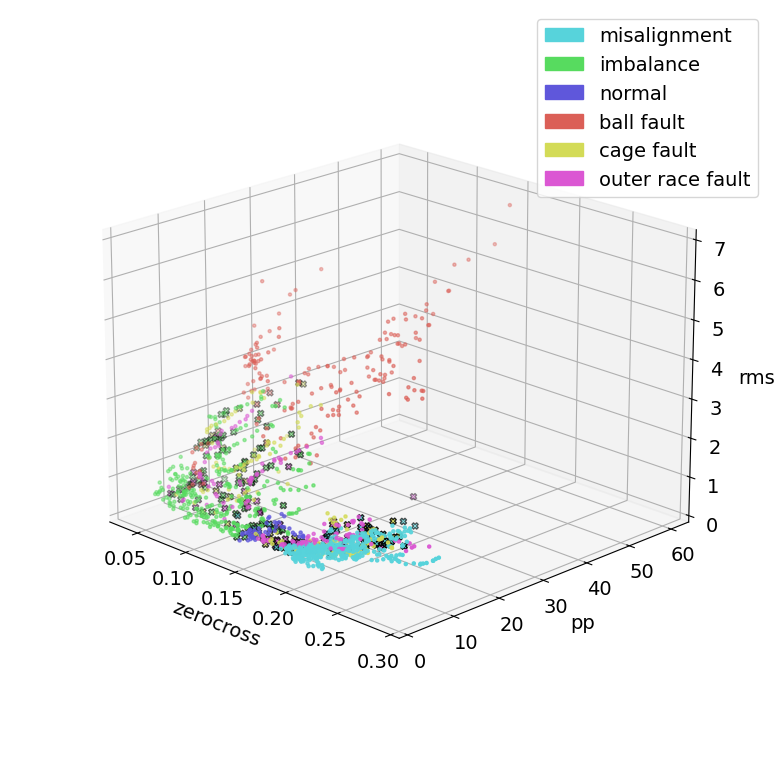
\includegraphics[width=\textwidth]{fig/scatter-mafaulda/td-rank-features.png}
         \caption{TD features (Accuracy = 83.90\%)}
     \end{subfigure}
     \hfill
     \begin{subfigure}[b]{0.45\textwidth}
         \centering
         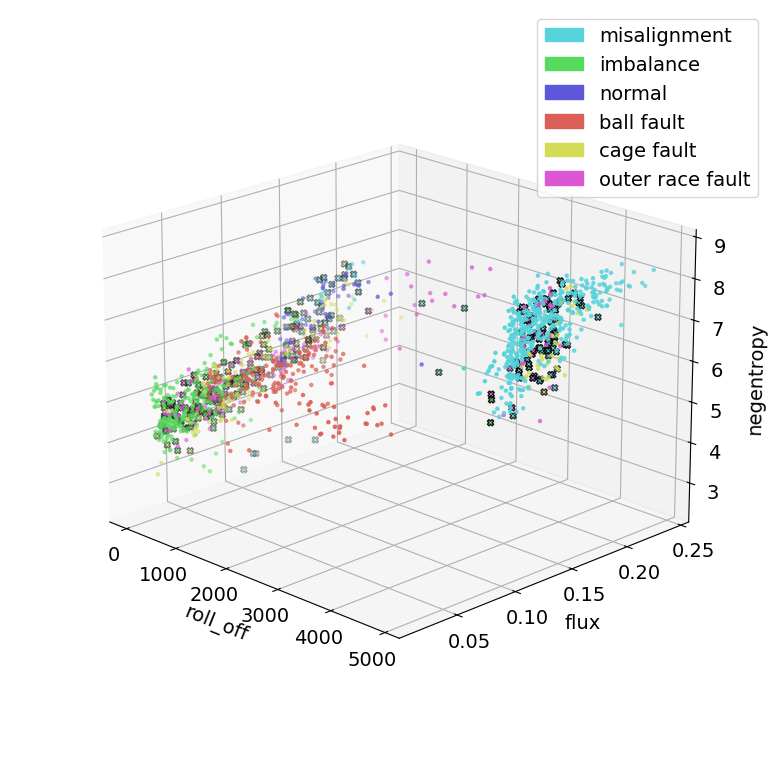
\includegraphics[width=\textwidth]{fig/scatter-mafaulda/fd-rank-features.png}
         \caption{FD features (Accuracy = 79.08\%)}
     \end{subfigure}
     \hfill
     \caption{Best 3 features for bearing A chosen by rank product}
     \label{tab:scatter-rank-product}
\end{figure}

The most commonly chosen subset of features by rank product are in order of decreasing popularity in the time domain: zero-crossing rate, root mean square, peak-to-peak, and in the frequency domain: roll-off frequency, centroid, flux, or entropy. Figure~\ref{tab:scatter-rank-product} shows clustering abilities of selected feature space for bearing A. Scale of attributes values are inverse of mix-max scaler function.

Features expressing machinery vibration amplitude, chaos, or richer frequency content look to be better predictors of fault types. The potential design of new features should follow these observations.

\section{Conclusions}
We reviewed processes and standards for vibration monitoring of rotating machinery using accelerometers. The aim is to diagnose faults of the machinery parts with a machine learning model and fewer features to make results more comprehensible. The related work includes low-level feature extraction as an important preprocessing step to reduce information from vibration signals. 

We built an embedded system with ESP32 MCU capable of recording vibrations from water pumps. Based on the data analysis of collected data, we discussed the problems with the implementation of a diagnostic model for machinery in the industry.

We developed the data pipeline with signal preprocessing and the k-nearest neighbors model for the MaFaulDa dataset. The bigger k values cause less accuracy for all feature spaces. Increasing the number of features taken out of the same feature set improves classification accuracy. The rank product balances the performance of other feature selection methods in the ensemble and reaches accuracies close to the upper quartile of the model distribution. 

The best validation accuracies found for one bearing when using just three features picked by rank product are 83.90\% (TD) and 79.08\% (FD). It is less than the accuracy for the best subset of three features by 1.82\% (TD), 5.13\% (FD), and is less than for the whole feature set. Relabeling faults to be only those with high severity gives an accuracy of three features for both bearings 89.96\% (TD) and 89.99\% (FD). Testing out different base feature sets could bring improvements for so few features.

\section*{Acknowledgements}
We thank Lukáš Doubravský (R-DAS,~s.r.o.) for consultations on the methodology and assisting in sensor unit development. We appreciate domain experts in vibrodiagnostics prof.~Stanislav Žiaran and Dr.~Ondrej Chlebo (SjF~STU) for checking our approches. We also thank Peter Csóka and Peter Kmeťko (Bratislavská vodárenská spoločnosť,~a.s.) for enabling us access to water pumps.

\printbibliography

\end{document}